%\documentclass[12pt, letterpaper]{book}
%\usepackage[margin=1in]{geometry} % layouts
% mobile phone layout
\documentclass[12pt, openany, a6paper]{book}
\usepackage[margin=5mm]{geometry} % layouts
% ipad layout
%\documentclass[12pt, a5paper, openany]{book}
%\usepackage[margin=5mm]{geometry} % layouts

\usepackage{titlesec} % custom chapter titles.
\usepackage{bibleref} % bible verse quoting
\usepackage{multicol} % two-column scripture readings
\usepackage{attrib} % bible verse quoting
\usepackage[hidelinks]{hyperref} % locating stuff
\usepackage{comment} % for conditional compilation
\usepackage{booktabs} % for a good table
\usepackage{graphicx} % for the logo
\usepackage{longtable} % for the scripture references that go too long
%\usepackage{lipsum} % fill in gaps for fomatting
%\usepackage{showframe} % layout
\usepackage{helvet} %arial for iphone

%----------------------------------------------------------
\renewcommand\familydefault{\sfdefault} % sans serif for digital

%----Begin Custom Title
\newcommand*{\wscoclogo}{
\includegraphics[height=1.5em]{walnutstcoc_logo_bw.png}} % Generic publisher logo
\newcommand*{\titleGM}{\begingroup % Create the command for including the title page in the document
\hbox{ % Horizontal box
\hspace*{0.08\textwidth} % Whitespace to the left of the title page
\rule{1pt}{\textheight} % Vertical line
\hspace*{0.04\textwidth} % Whitespace between the vertical line and title page text
\parbox[b]{0.8\textwidth}{ % Paragraph box which restricts text to less than the width of the page

{\noindent\LARGE\bfseries ``For They Shall All Know Me''}

\vspace{0.5\baselineskip}

{\Large \textit{Developing a New Covenant Relationship with God}}

\vspace{1\baselineskip}

\vspace{1\baselineskip}%{\noindent\LARGE TEACHERS MANUAL}

\vspace{4\baselineskip}

{\Large \textsc{Todd Jobe}} % Author name

\vspace{0.5\textheight} % Whitespace between the title block and the publisher

{\noindent Walnut Street Church of Christ \wscoclogo}

\vspace{0.5\baselineskip} % Publisher and logo
}}
\endgroup}
%----End Custom Title
%---------Old Title----------------------------------------------------------
%\title{``For They Shall All Know Me''\\\Large{Developing a New Covenant Relationship with God}\\\LARGE\uppercase{TEACHERS MANUAL}}
%\author{Walnut Street Church of Christ\\Todd Jobe}
%\date{Spring 2016}
%----------------------------------------------------------


\renewcommand\chaptername{Lesson}

% sectioning with conditional compilation using specialcomment
% if you don't want to include a section just follow this portion with
% \excludecomment{nameofsection}
\specialcomment{intro}{\section*{Introduction}}{}
\specialcomment{bible}{
\section*{Scripture Readings}
%\begin{multicols}{2}
}
{
%	\end{multicols}
}
\specialcomment{goals}{
	\begingroup
	\newcommand{\goal}{\item}
	
	\section*{Goals}
	
	\begin{itemize} \itemsep1pt \parskip0pt \parsep0pt
	
}
{
	\end{itemize}
	\endgroup
}
\specialcomment{discussion}{\section*{Discussion}}{}
\specialcomment{questions}{
	\begingroup
	\newcommand{\q}{\item}
	
	\clearpage
	
	\section*{Questions}
	
	\begin{enumerate}
	
}
{
	\end{enumerate}
	\endgroup
}
%\newcommand{scriptRefTab}{\begin{tabular}{lrp{11cm}}}
%\newcommand{scriptRefTab}{\begin{longtable}{lrp{0.68\textwidth}}}
%\newcommand{scriptRefTab}{\begin{longtable}{lrp{0.55\textwidth}}}

\newenvironment{scriptref}{
	\begingroup
	\begin{center}
	%\begin{tabular}{lrp{11cm}} % book
	%\begin{longtable}{lrp{0.66\textwidth}} % tablet
	\begin{longtable}{lrp{0.55\textwidth}} % iphone
}
{
	\end{longtable} % digital
	%\end{tabular} % print
	\end{center}
	\endgroup
}
%\excludecomment{goals}
\excludecomment{intro}
%\excludecomment{bible}
\excludecomment{discussion}
%\excludecomment{questions}
\renewcommand{\labelitemi}{--} % better start to lists.
\newcommand\dsubsec[3]{\subsection*{#1 \normalsize{(#2, #3 min)}}} % discussion subsection
%\newcommand\questions{\section*{Questions}} 
\newcommand\bv[2]{\subsubsection*{\bibleverse{#1}#2}} % bible vers in Scripture Readings section
\newcommand\bve[2]{\subsubsection*{\bibleverse{#1}#2~\scriptsize{(ESV)}}} % bible vers in Scripture Readings section
\newcommand\bvh[2]{\subsubsection*{\bibleverse{#1}#2~\scriptsize{(HCSB)}}\label{bv:#1#2}} % bible vers in Scripture Readings section
\newcommand\bvs[2]{\emph{\bibleverse{#1}#2} -- } % bible verse intext reference

% chapter format
\titleformat{\chapter}[hang] 
{\normalfont\Large\bfseries}{\chaptertitlename\ \thechapter:}{0.2em}{} 
\titlespacing*{\chapter}{0pt}{-20pt}{10pt}

% sectioning formats
\titleformat{\section}
{	\normalfont\large\bfseries}{\thesection}{.5em}{}[{\titlerule[0.8pt]}]
\titleformat{\subsection}
{\normalfont\normalsize\bfseries}{\thesubsection}{.5em}{}
\titleformat{\subsubsection}
{\normalfont\normalsize\bfseries}{\thesubsubsection}{.5em}{}
\titleformat{\paragraph}[runin]
{\normalfont\normalsize\bfseries}{\theparagraph}{.5em}{}
\titleformat{\subparagraph}[runin]
{\normalfont\normalsize\bfseries}{\thesubparagraph}{.5em}{}

\begin{document}
\pagestyle{plain}
\frontmatter

% --- Old Title
%\maketitle
% --- Custom Title
\thispagestyle{empty} % Removes page numbers from title page
\titleGM % This command includes the title page
% --- 
\clearpage
~\vfill
\begin{center}
Scripture quotations marked (ESV) are from the ESV\textsuperscript{\textregistered}. Bible (The Holy Bible, English Standard Version\textsuperscript{\textregistered}.), copyright \textcopyright~2001 by Crossway, a publishing ministry of Good News Publishers. Used by permission. All rights reserved.

\vspace{2em}

Scripture quotations marked (HCSB), are taken from the Holman Christian Standard Bible\textsuperscript{\textregistered}, Copyright \textcopyright~1999, 2000, 2002, 2003, 2009 by Holman Bible Publishers. Used by permission. HCSB\textsuperscript{\textregistered} is a federally registered trademark of Holman Bible Publishers.
\end{center}
\clearpage

\tableofcontents

%\cleardoublepage
%\section*{Theme}
%\addcontentsline{toc}{chapter}{Theme}
\chapter{Theme}
\begin{center}
\Large God wants a relationship with people.
\end{center}

\section*{Key Passage}\label{sec:KeyPassage}

\begin{quote}
31 ``Behold, the days are coming, declares the Lord, when I will make a new covenant with the house of Israel and the house of Judah, 32 not like the covenant that I made with their fathers on the day when I took them by the hand to bring them out of the land of Egypt, my covenant that they broke, though I was their husband, declares the Lord. 33 For this is the covenant that I will make with the house of Israel after those days, declares the Lord: I will put my law within them, and I will write it on their hearts. And I will be their God, and they shall be my people. 34 And no longer shall each one teach his neighbor and each his brother, saying, `Know the Lord,' for they shall all know me, from the least of them to the greatest, declares the Lord. For I will forgive their iniquity, and I will remember their sin no more.'' \attrib{Jeremiah 31:31-34, ESV}
\end{quote}

\section*{Class Objectives}\label{sec:ClassObjectives}
\begin{itemize}
\item Know the big picture of the Bible:\\\emph{God wants a relationship with a holy people who voluntarily choose Him}
\item Understand how the ``relationship'' theme develops from the Old Covenant to the New Covenant.
\item Develop a ``relationship'' perspective in your own walk with God.
\end{itemize}


\clearpage
%\csname @openrightfalse\endcsname % for print only
\chapter{Scripture Reference}

\begin{scriptref}
\toprule
\multicolumn{3}{l}{\large Old Testament}\\
%\endfirsthead
Passage & Ls. & Message \\
\midrule
%\endhead
Gen. 2:20-24    & 5  & Husband and wife relationship is a very close bond\\
Gen. 6:17-18    & 4  & God made a covenant with Noah \\
Gen. 22:15-19   & 7  & Land, nation, seed promises to Abraham\\
Gen. 17:1-8     & 2  & ``I will be your God'' to Abraham\\
Ex. 6:1-9       & 1  & ``I will be your God'' to the Israelites\\
Lev. 22:31-33   & 1  & ``I am holy'', ``I am your God'', to the Israelites\\
Lev. 26:1-45    & 6  & Israel's consequences for rejecting God\\
Deut. 10:12-22  & 3  & The Lord set aside a special people whos' hearts are His\\
I Sam. 16:7     & 9  & Man looks at the outward appearance.  God looks at the heart.\\
Ezra 7:10       & 9  & Ezra chose what his heart would be like.\\
Psalm 8:1-9     & 2  & What is man that You are mindful of him?\\
Eccl. 3:11      & 2  & We know God because He set eternity in our heart\\
Jer. 31:31-34   & 1  & Prophecy of the New Covenant\\
Ezek. 37:1-28   & 3  & Dry bones \& ``I will be their God.  They shall be my people''\\
\bottomrule
\end{scriptref}
%\clearpage
\begin{scriptref}
\toprule
\multicolumn{3}{l}{\large New Testament}\\
Passage & Ls. & Message \\
\midrule
\endhead
Matt. 7:7-12    & 10 & Keep asking and it will be given you.\\
Matt. 20:1-16   & 11 & Whether you come to God early or late, the reward is fixed.\\
Matt. 22:1-14   & 3  & You can refuse the Lord's offer of a relationship\\
Luke 2:22-40    & 7  & Simeon and Anna, two Israelites, were expecting Jesus\\
Luke 4:1-13     & 2  & Jesus rebuffs Satan by using God as His moral anchor\\
Luke 14:25-27   & 2  & Loving God is the key to eternal life\\
Luke 22:14-23   & 8  & Jesus' blood is the seal of the New Covenant\\
John 3:16       & 1  & God's love is His motivation for our salvation\\
Rom. 3:5-31     & 12 & Everyone is under sin, so that God may have mercy on all.\\
Rom. 4:1-25     & 10 & Those who have the faith of Abraham are his children.\\
Rom. 7:1-25     & 12 & Paul illustrates the impossibility perfect law keeping.\\
Rom. 8:1-11     & 12 & There is no condemnation of sin for those in Christ Jesus.\\
Rom. 8:12-17    & 3  & God adopts us as sons.\\
Rom. 8:18-23    & 7  & Christians are still waiting for their coming glory.\\
Rom. 8:28-30    & 3  & The Lord predestined the type of people who would be his\\
Rom. 9:30-33    & 6  & Israel didn't have faith and, so, stumbled over Jesus.\\
Rom. 11:25-32   & 8  & God shut everyone up under sin, so He can show mercy.\\
Rom. 12:1-2     & 9  & Christians commit to a total life transformation.\\
II Cor. 3:7-18  & 8  & The temple veil has been removed.  So we know God directly.\\
II Cor. 4:16-18 & 9  & The outer person fades, but the inner person is renewed.\\
Gal. 3:1-29     & 4  & Faith is the foundation of God's covenants\\
Eph. 2:1-21     & 8  & Jews and Gentiles are reconciled to God through Christ.\\
Eph. 3:1-6      & 11 & The mystery of the Gospel is that Gentiles can enter heaven.\\
Eph. 3:14-18    & 10 & Our heart is strengthened as we grow in knowing God's love.\\
Eph. 4:1-16     & 11 & Christians are each part of a body, and work toward unity.\\
Phil. 3:3-10    & 10 & We are the true circumcision, and we focus on knowing Christ.\\
Heb. 1:1-2      & 2  & We know God because He spoke by the prophets and His Son\\
Heb. 3:1-19     & 6  & Israel hardened their hearts to God.  Don't harden yours.\\
Heb. 4:1-13     & 9  & Don't have the Israel's heart, rather faith guided by the Word.\\
Heb. 8:1-13     & 1  &  The Old Covenant had faults and is replaced with the New\\
Heb. 9:1-14     & 11 & Jesus entered a spiritual Holy Place to bring true redemption.\\
Heb. 9:15-28    & 12 & Jesus is the solution to the problem of sin.\\
Heb. 10:1-23    & 8  & Jesus' sacrifice forgives and sanctifies, once for all.\\
Heb. 12:1-29    & 5  & God's discipline and the greatness of his plan motivates us\\
James 2:1-7     & 11 & The church has both rich and poor and they should get along.\\
I Pet. 2:9-10   & 3  & The Lord's people are a chosen race and a royal priesthood\\
I John 4:7-12   & 5  & Love is the main characteristic of God \ldots and Christians\\
I John 3:19-24  & 9  & A heart that has love and obedience gives us confidence.\\
\bottomrule
\end{scriptref}

\mainmatter

\lecture{Introduction}{01-Introduction}
% - Exactly two or three sections (other than the summary).
% - At *most* three subsections per section.
% - Talk about 30s to 2min per frame. So there should be between about
%   15 and 30 frames, all told.

\section{Introduction}

\begin{goals}
\goal Become familiar with the class theme, key passage, and class objectives.
\goal Understand how each subsequent lesson fits into the class objectives.
\goal Do an initial evaluation of how relationship-focused your religion is.
\end{goals}

\begin{frame}
\begin{quote}
31 Behold, the days are coming, declares the Lord, when I will make a new covenant with the house of Israel and the house of Judah, 32 not like the covenant that I made with their fathers on the day when I took them by the hand to bring them out of the land of Egypt, my covenant that they broke, though I was their husband, declares the Lord. 33 For this is the covenant that I will make with the house of Israel after those days, declares the Lord: I will put my law within them, and I will write it on their hearts. And I will be their God, and they shall be my people. \attrib{Jeremiah 31:31-33}
\end{quote}
\end{frame}

%\begin{discussion}
%\dsubsec{Introduction}{900-905}{5}
%
%This lesson is about who God is.
%
%\bvs{Genesis}{(17:1-8)} God's first covenant with Abraham says that he will be his God.
%
%\dsubsec{Who is God?}{905-915}{10}
%
	%\bvs{Psalms}{(8:1-9)} It's amazing that God is is mindful of us.
%
%\dsubsec{How we come to know about God}{915-925}{10}
%
	%\bvs{Ecclesiastes}{(3:11)} Eternity in the heart of man
%
  %\bvs{Hebrews}{(1:1-2)} Fathers by the prophets, today His son
	%
	%By extension His Word.
%
%\dsubsec{What does that mean for me?}{925-940}{15}
%
	%\bvs{Luke}{(4:1-13)} Having a God gives you an anchor. 
	%
	%\bvs{Luke}{(14:25-27)} Love God and you will live.
%
%\dsubsec{Review}{940-945}{5}
%\end{discussion}

%\begin{frame}{Class Theme}{Subtitles are optional.}
  %% - A title should summarize the slide in an understandable fashion
  %%   for anyone how does not follow everything on the slide itself.
%
  %\begin{itemize}
  %\item
    %Use \texttt{itemize} a lot.
  %\item
    %Use very short sentences or short phrases.
  %\end{itemize}
%\end{frame}
%\begin{frame}{Lesson Motivation}{Subtitles are optional.}
  %% - A title should summarize the slide in an understandable fashion
  %%   for anyone how does not follow everything on the slide itself.
%
  %\begin{itemize}
  %\item
    %Use \texttt{itemize} a lot.
  %\item
    %Use very short sentences or short phrases.
  %\end{itemize}
%\end{frame}
%\begin{frame}{Lesson Objectives}{Subtitles are optional.}
  %% - A title should summarize the slide in an understandable fashion
  %%   for anyone how does not follow everything on the slide itself.
%
  %\begin{itemize}
  %\item
    %Use \texttt{itemize} a lot.
  %\item
    %Use very short sentences or short phrases.
  %\end{itemize}
%\end{frame}
%\section{Point1}
%\section{Point2}
%\section{Point3}
%\subsection[Objectives]{Theme}
%\subsection[Short First Subsection Name]{First Subsection Name}
%
%\begin{frame}{Make Titles Informative. Use Uppercase Letters.}{Subtitles are optional.}
  %% - A title should summarize the slide in an understandable fashion
  %%   for anyone how does not follow everything on the slide itself.
%
  %\begin{itemize}
  %\item
    %Use \texttt{itemize} a lot.
  %\item
    %Use very short sentences or short phrases.
  %\end{itemize}
%\end{frame}
%
%\begin{frame}{Make Titles Informative.}
%
  %You can create overlays\dots
  %\begin{itemize}
  %\item using the \texttt{pause} command:
    %\begin{itemize}
    %\item
      %First item.
      %\pause
    %\item    
      %Second item.
    %\end{itemize}
  %\item
    %using overlay specifications:
    %\begin{itemize}
    %\item<3->
      %First item.
    %\item<4->
      %Second item.
    %\end{itemize}
  %\item
    %using the general \texttt{uncover} command:
    %\begin{itemize}
      %\uncover<5->{\item
        %First item.}
      %\uncover<6->{\item
        %Second item.}
    %\end{itemize}
  %\end{itemize}
%\end{frame}
%
%
%\subsection{Second Subsection}
%
%\begin{frame}{Make Titles Informative.}
%\end{frame}
%
%\begin{frame}{Make Titles Informative.}
%\end{frame}
%
%
%
%\section*{Summary}
%
%\begin{frame}{Summary}
%
  %% Keep the summary *very short*.
  %\begin{itemize}
  %\item
    %The \alert{first main message} of your talk in one or two lines.
  %\item
    %The \alert{second main message} of your talk in one or two lines.
  %\item
    %Perhaps a \alert{third message}, but not more than that.
  %\end{itemize}
  %
  %% The following outlook is optional.
  %\vskip0pt plus.5fill
  %\begin{itemize}
  %\item
    %Outlook
    %\begin{itemize}
    %\item
      %Something you haven't solved.
    %\item
      %Something else you haven't solved.
    %\end{itemize}
  %\end{itemize}
%\end{frame}


\lecture{2. I will be their God}{02}

\section*{Introduction}

\begin{frame}
\frametitle{Texas is my state}
	\begin{center}
	
\includegraphics[width=.9\textwidth]{figures/texas.jpg}
	\end{center}
\note{09:30}
\note[item]{I, like most Texans, am proud where I come from.}
\note[item]{Texans are taught that their state is simply better than any other state (or country).}
\note[item]{God wants us to think that way about Him -- that He is simply better.}
\note[item]{He is the only one that deserves our loyalty.}
\note[item]{He wants His team to be the only team we play for.}
\end{frame}

\begin{frame}
\frametitle{God wants a relationship with people}
\framesubtitle{Jeremiah 31:31-34}
	\keyversehiglight{I will be their God}
	\note{09:32}
	\note[item]{In our class we're trying to establish, from the Bible, the idea that God 
wants a relationship with people.}
	\note[item]{We're using Jeremiah 31:31-34 as a means of focusing that study.}
	\note[item]{Jeremiah 31:31-34 is one of the most important passages in the Bible, because it provides a connection between the old covenant and the new covenant, and talks about the close, special relationship that God's chosen people have with Him.  Under the old covenant, those people were the Israelites.  Under the New Covenant, those special people are all Christians.}
	\note[item]{\emph{Read it}}
	\note[item]{Today we'll be talking about how God wants to be the only God in our lives.}
\end{frame}

\begin{goals}
\goal Consider who God is, and consider how He is similar and different from man.
\goal Explore the different ways God has revealed himself to man.
\goal Think about ways to improve my perspective on who God is.

\note{09:33}
\note[item]{Examine why God is worthy of our loyalty.}
\note[item]{Examine how we learn about God's greatness.}
\note[item]{Considering how we can increase our devotion to God.}
\end{goals}

\section{I will be your God}

\begin{frame}
\frametitle{I will be your God}
\framesubtitle{Gen 17:1-8}
\begin{columns}[T]
	\begin{column}{0.4\textwidth}
		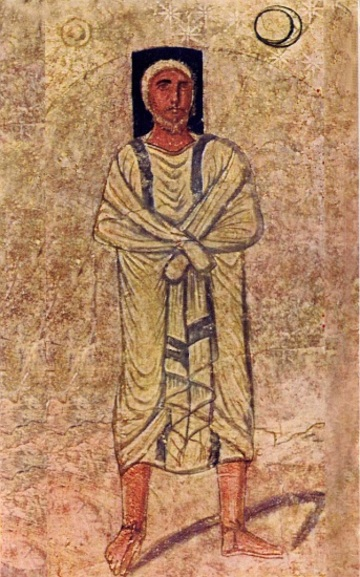
\includegraphics[height=0.8\textheight]{figures/abrahamDuraEuropos.jpg}
	\end{column}
	\begin{column}{0.6\textwidth}
		``And I will give you and to your offspring after you the land of your sojournings, all the land of Canaan, for an everlasting possession, and \\\alert{I will be their God}.'' -- Genesis 17:8
	\end{column}
\end{columns}

\note{09:35}
\note[item]{God recounts his 3-fold promise to Abraham: land, nation, seed (if you count ``kings shall come from you'')}.
\note[item]{Part or all of these promises are repeated at various times in Abraham's life (Gen 12, 13, 15, 17, 22)}
\note[item]{The first occurrence of the phrase `I will be their God' is in God's promise to Abraham.}
\note[item]{Fresco pictured here is one of the earliest depictions of a Bible narrative.  It depicts Abraham and God's promises to Him.  It is from the Dura-Europos synagogue 244 AD  70\% of the city has been destroyed during the Syrian civil war.}
\note[item]{When does God mean when he says `I will be their God'? \emph{Abraham had many `gods' to choose from, but God wanted Abraham to love only Him.}}
\note[item]{vs.1-2 Because God is mighty, he had to put a condition on His covenant with Abraham -- be blameless.}
\end{frame}

\begin{frame}
\frametitle{`I will be their God' through the Bible}
\begin{columns}[T]
	\begin{column}{0.45\textwidth}
		`I will be their God'\\{\footnotesize Gen. 17:8, Jer. 24:7, Jer. 31:33\\Jer. 32:36, Jer. 32:38, Ez. 11:20\\Ez. 37:15, Ez. 37:23, Ez. 37:27\\Zech. 8:8, 2 Cor. 6:16, Heb. 8:10}\\~\\
		`I will be your God'\\{\footnotesize Ex. 6:7, Jer. 7:23, Jer. 11:4\\Jer. 30:2, Ez. 36:28}\\~\\
	\end{column}
	\begin{column}{0.55\textwidth}
			`the Lord your God'\\ 
			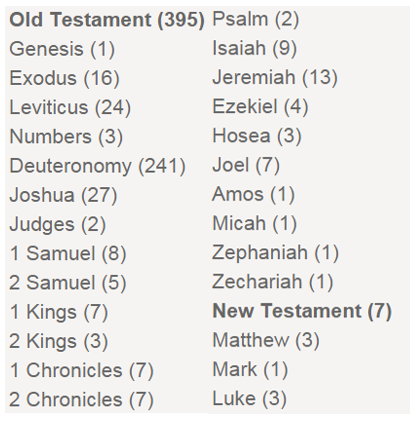
\includegraphics[width=1\columnwidth]{figures/theLordYourGodTwoColumn.png}
	\end{column}
\end{columns}

\note{09:38}
\note[item]{Last week, `your God', given to the Israelites as part of the Law of Moses (Ex. 6:1-9, Lev. 22:31-33).}
\note[item]{Clearly God thinks it's important that we view Him as the only God.}
\note[item]{It's not just that His people accept Him as the `true' God.  But as `their' God}
\end{frame}

\section{Who is God?}

\begin{frame}
\frametitle{God is majestic}
\framesubtitle{Psalm 8}
\begin{center}
	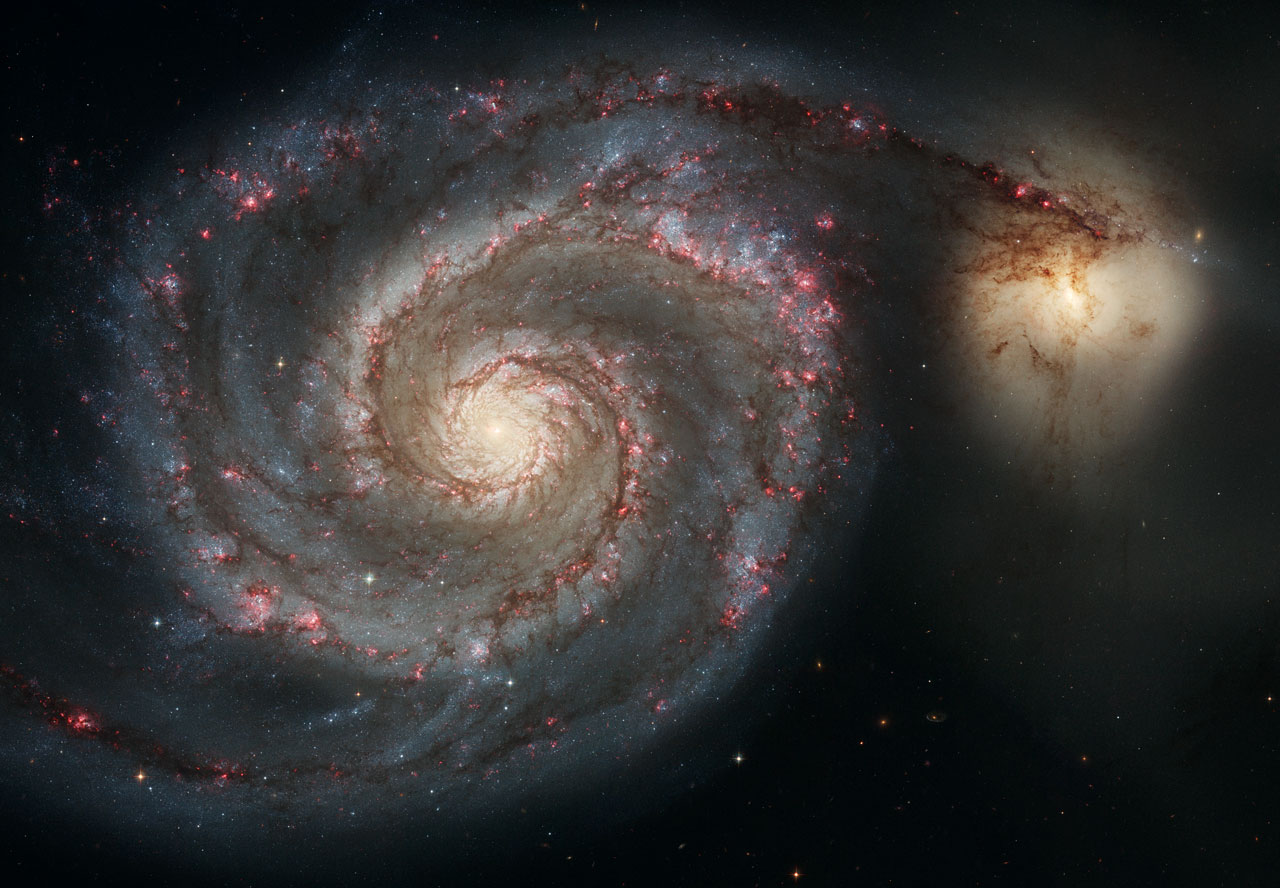
\includegraphics[width=0.85\textwidth]{figures/galaxy.jpg}\\
	{\footnotesize The Whirlpool galaxy as seen from the Hubble Space Telescope}
\end{center}

\note{09:40}
\note[item]{The Whirlpool galaxy is 60,000 LY across.  You can see it clearly with your own telescope.  Right below the handle of the big dipper.}
\note[item]{I'm small compared to God.}
\end{frame}

\begin{frame}
\frametitle{Man is not the source of God's greatness}
\framesubtitle{Psalm 8}
Out of the mouth of babes and sucklings hast thou perfected praise, because of thine enemies; that thou mightest put down the enemy and avenger.\hfill--Psalm 8:2 (LXX)\\~\\
15 But when the chief priests and the scribes saw the wonderful things that he did, and the children crying out in the temple, ``Hosanna to the Son of David!'' they were indignant, 16 and they said to him, ``Do you hear what these are saying?'' And Jesus said to them, ``Yes; have you never read,
\begin{quote}
`Out of the mouth of infants and nursing babies you have prepared praise'?
\end{quote}\\
\hfill-- Matt. 21:15-16 (ESV)
\normalsize

\note{09:41}
\note[item]{In context, Psalm 8:2 may refer to Israel, who followed the true God, being small and the surrounding nations being `great'.}
\note[item]{Jesus quotes Psalm 8:2 to remind the chief priests and scribes that they are not the source of His approval.}
\note[item]{It's important to remember that God is great, whether or not man accepts it.}
\end{frame}

\begin{frame}
\frametitle{God loves man and has blessed him.}
\framesubtitle{Psalm 8}
\begin{center}
	
\includegraphics[width=\textwidth]{figures/manLandscape.jpg}\\
	``The worst moment for the atheist is when he is really thankful and has nobody to thank.''
\end{center}

\note{09:45}
\note[item]{Man is not powerful like God is.}
\note[item]{Yet, He has made us special compared to all other creation}
\note[item]{Man is special and loved even when he rejects God.}
\note[item]{Quote is possibly attributed to Dante Gabriel Rossetti, a painter poet from the mid-19th century}
\end{frame}

\section{How we come to know about God}

\begin{frame}
\frametitle{Eternity is set in the heart of man}
\framesubtitle{Ecclesiastes 3:11}

\includegraphics[width=\textwidth]{figures/eternityInHeart.jpg}

\note{09:48}
\note[item]{God has always made Himself known to man}
\note[item]{What does the passage mean? \emph{Man innately understands the possibility that something could exist beyond his own world.}}
\note[item]{However God may have chosen to speak to us, He was always going to leverage that part of our being that understands there's something more to life.}
\note[item]{Romans 1 -- Creation speaks to an `un-caused cause', which should lead us to consider God.}

\end{frame}

\begin{frame}
	\frametitle{In the past, God spoke to the Fathers by the prophets}
	\framesubtitle{Hebrews 1:1-2}
	\begin{center}
	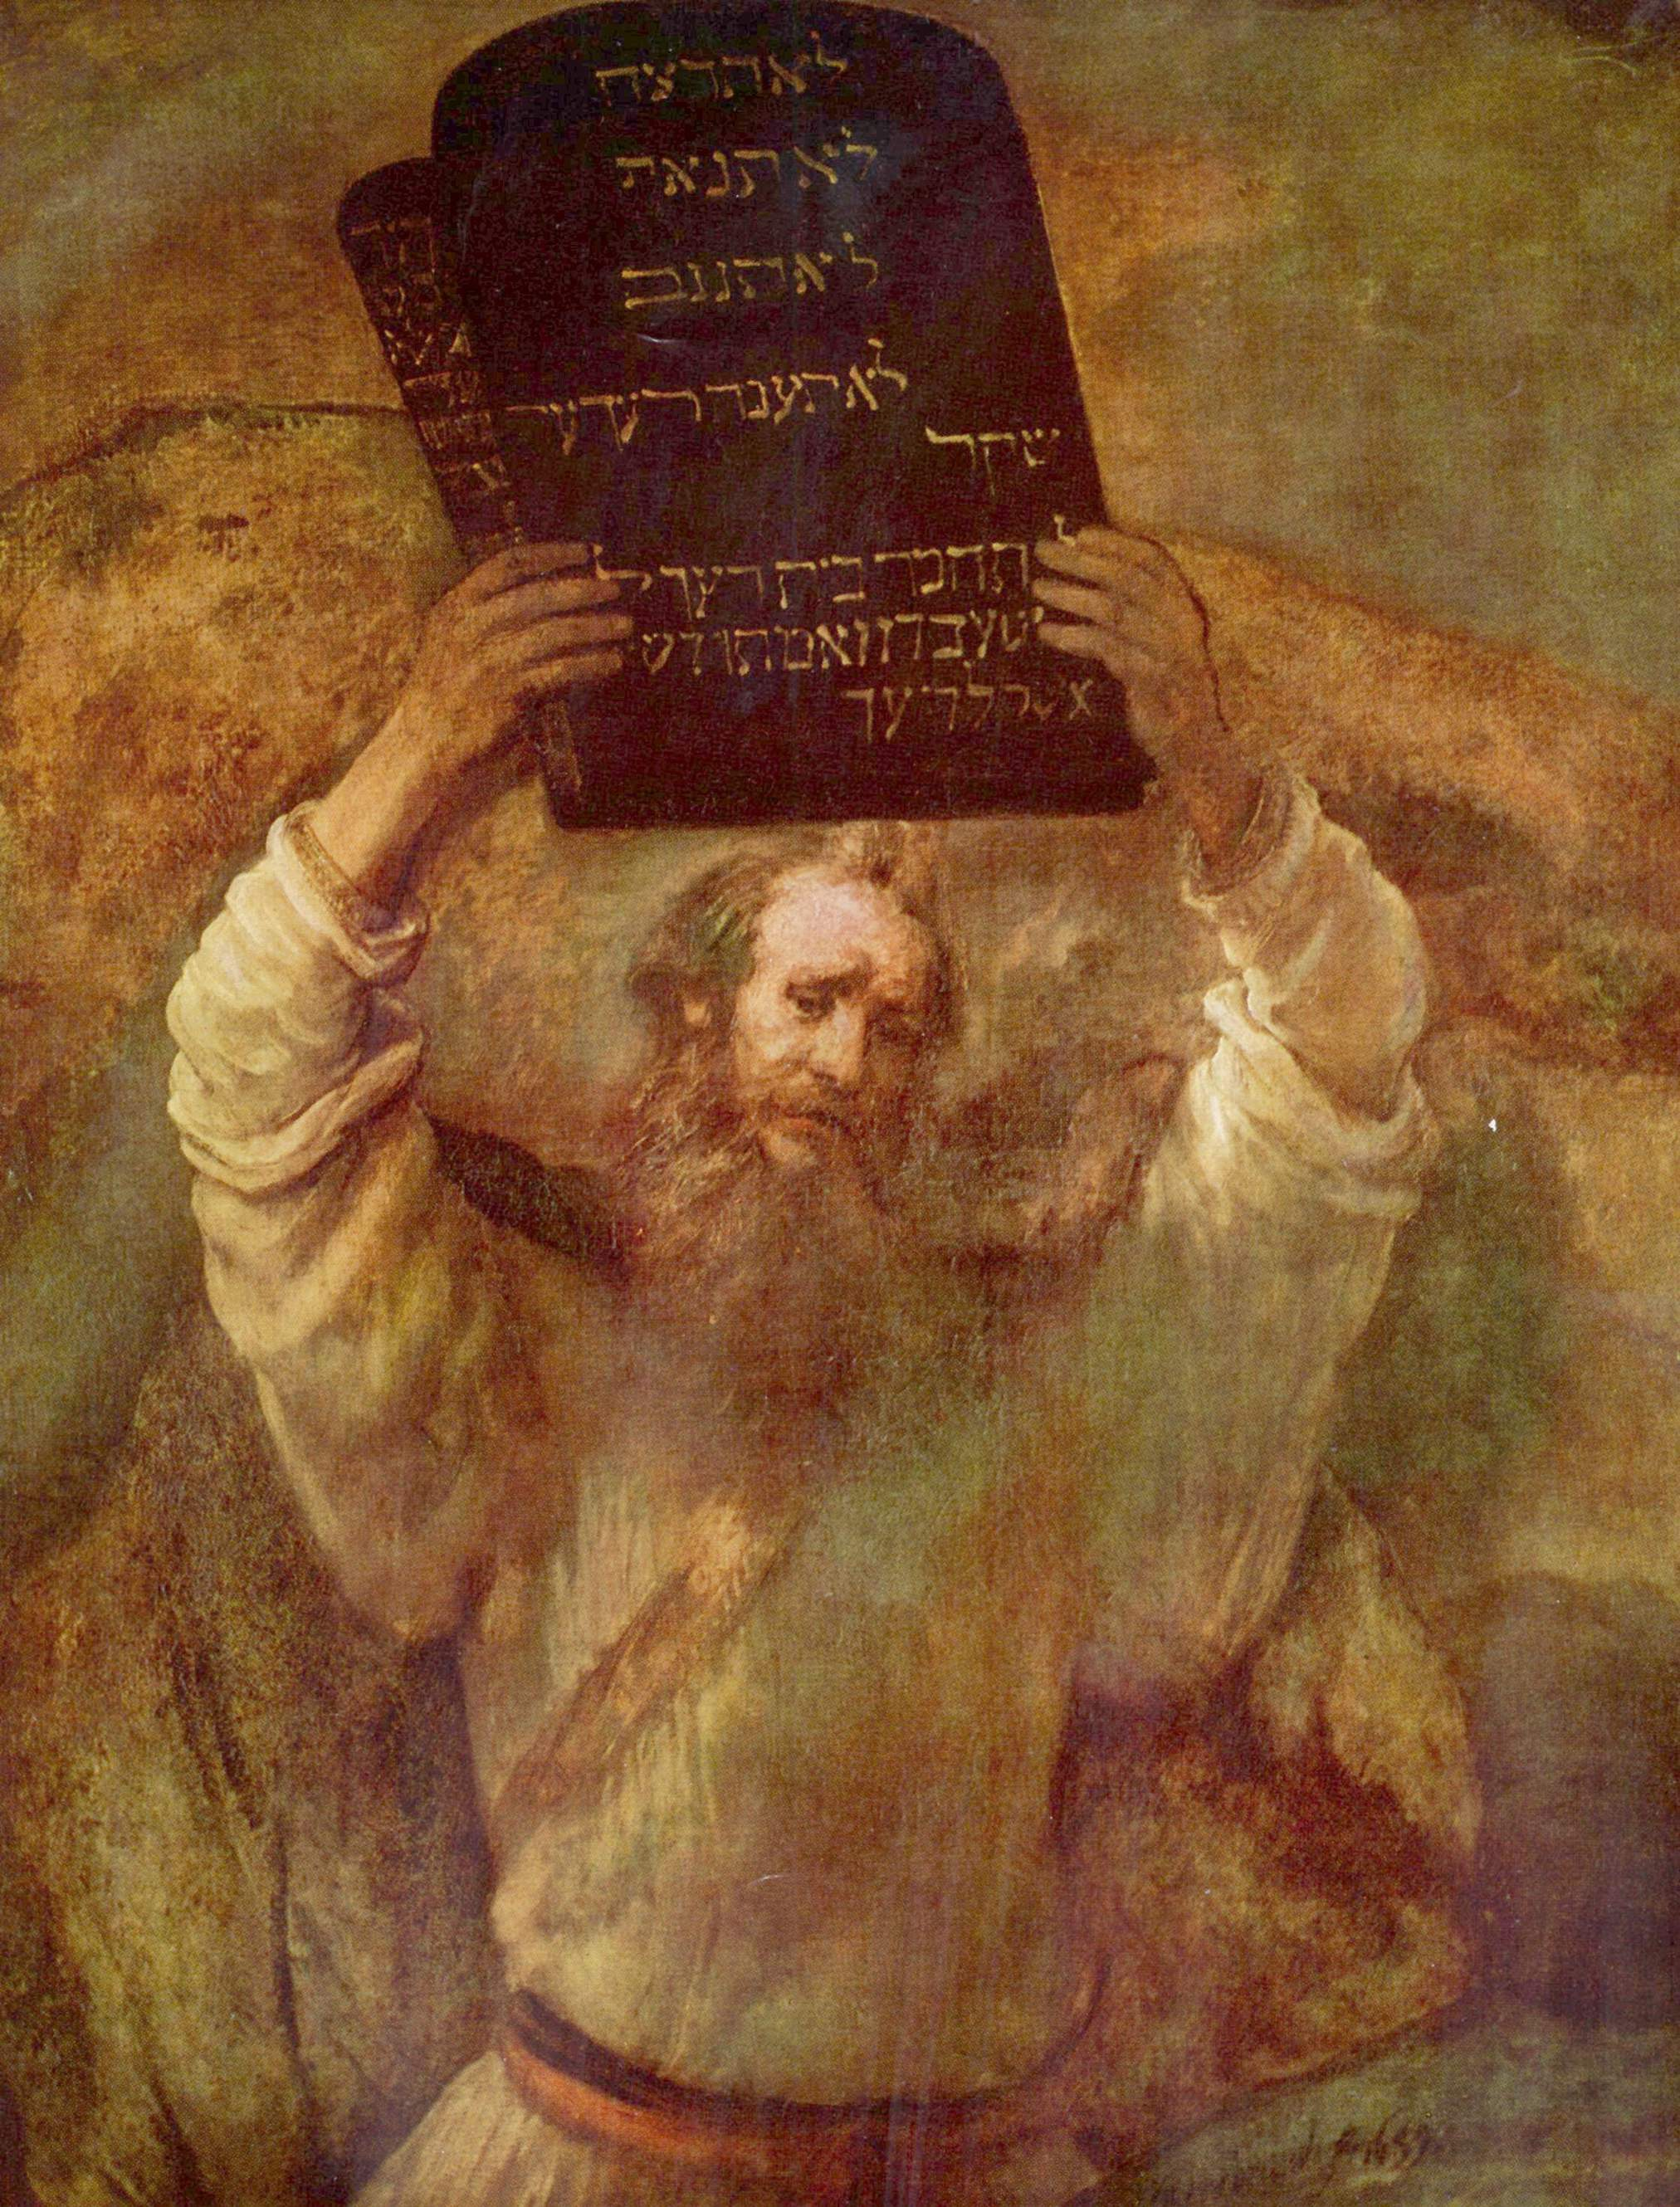
\includegraphics[height=0.8\textheight]{figures/mosesTenCommandments.jpg}
	\end{center}
	
	\note{09:50}
	\note[item]{The Israelites would have viewed Moses as the greatest prophet, the giver of God's Law.}
	\note[item]{Prophets would also include all those people we normally think of as prophets, whose main purpose was to plead for Israel to repent from wickedness.}
	\note[item]{The author leaves out the patriarchs. But, remember, he's just trying to make a point.}
	\note[item]{What's tough about learning from prophets? \emph{People don't have access to prophets all the time.  And, prophets just `tell' you what perfect faithfulness looks like.  They can't `show' you what perfect faithfulness looks like.}}
	\note[item]{Painting:Rembrandt}
\end{frame}

\begin{frame}
	\frametitle{Today, God speaks to us in His Son, Jesus}
	\framesubtitle{Hebrews 1:1-2}
	\begin{center}
	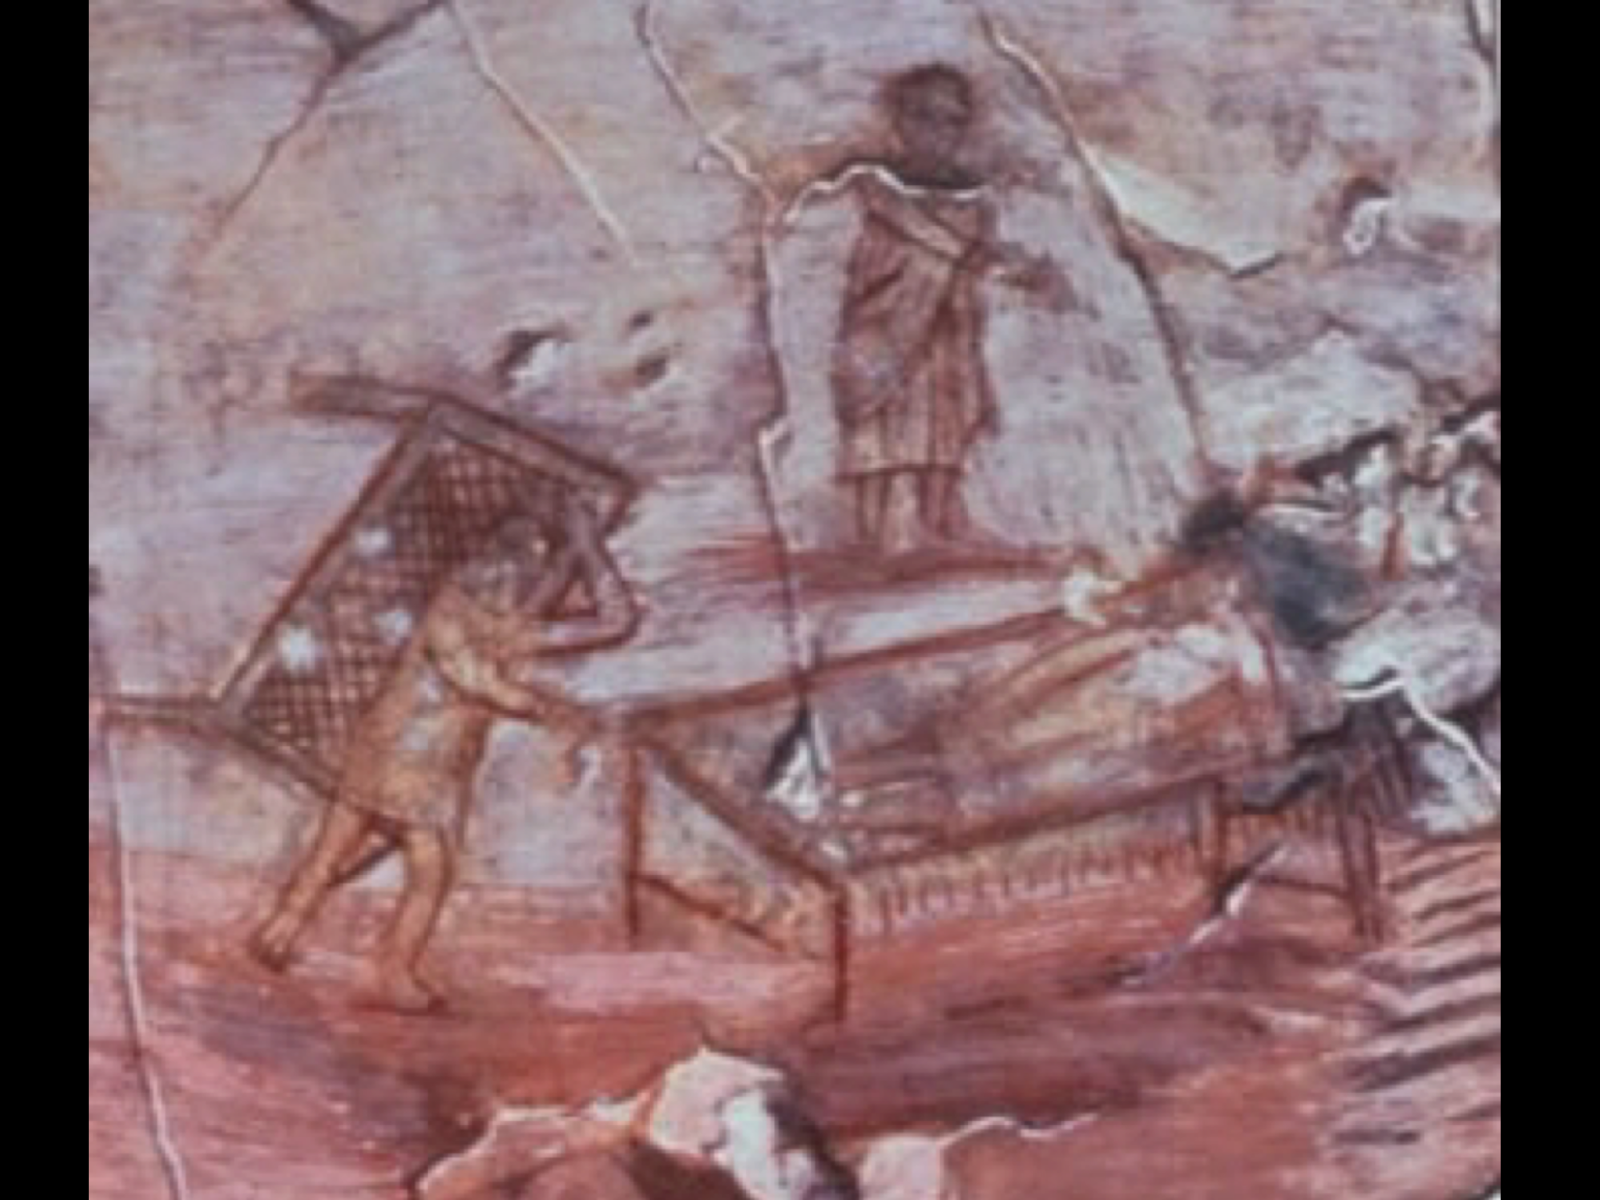
\includegraphics[height=0.8\textheight]{figures/jesusHealingParalytic.png}
	\end{center}
	
	\note{09:53}
	\note[item]{Speak means much more than simply teaching.}
	\note[item]{Jesus' life itself was God showing us how to live righteous.}
	\note[item]{God was under no obligation to do this.  He loved us.}
	\note[item]{But, even with Jesus, you only had direct access to his life if you lived in 1st century Palestine.}
	\note[item]{The fresco pictured is also from Dura-Europos (225AD), but a church instead of a synagogue.  It pictures Jesus healing the paralytic.  It's the earliest known depiction of Jesus.  In general, early Christians did not make images of Jesus.}
\end{frame}

\begin{frame}
	\frametitle{...And by extension His Word}
	\framesubtitle{Hebrews 1:1-2}
	\begin{center}
	
\includegraphics[width=\textheight]{figures/godSpeaksThroughTheWord.jpg}
	\end{center}
	
	\note{09:57}
	\note[item]{God has always shown Himself to man, but never more easily and more clearly than today}
	\note[item]{The Bible doesn't change through time.}
	\note[item]{The Bible is easily available for most people.}
	\note[item]{God makes himself `our God' when we read His word, understand it, and believe it}.
\end{frame}

\section{What does that mean for me?}

\begin{frame}
	\frametitle{God gives you moral anchor}
	\framesubtitle{Luke 4:1-13}
	\begin{columns}
	\begin{column}{0.5\textwidth}
	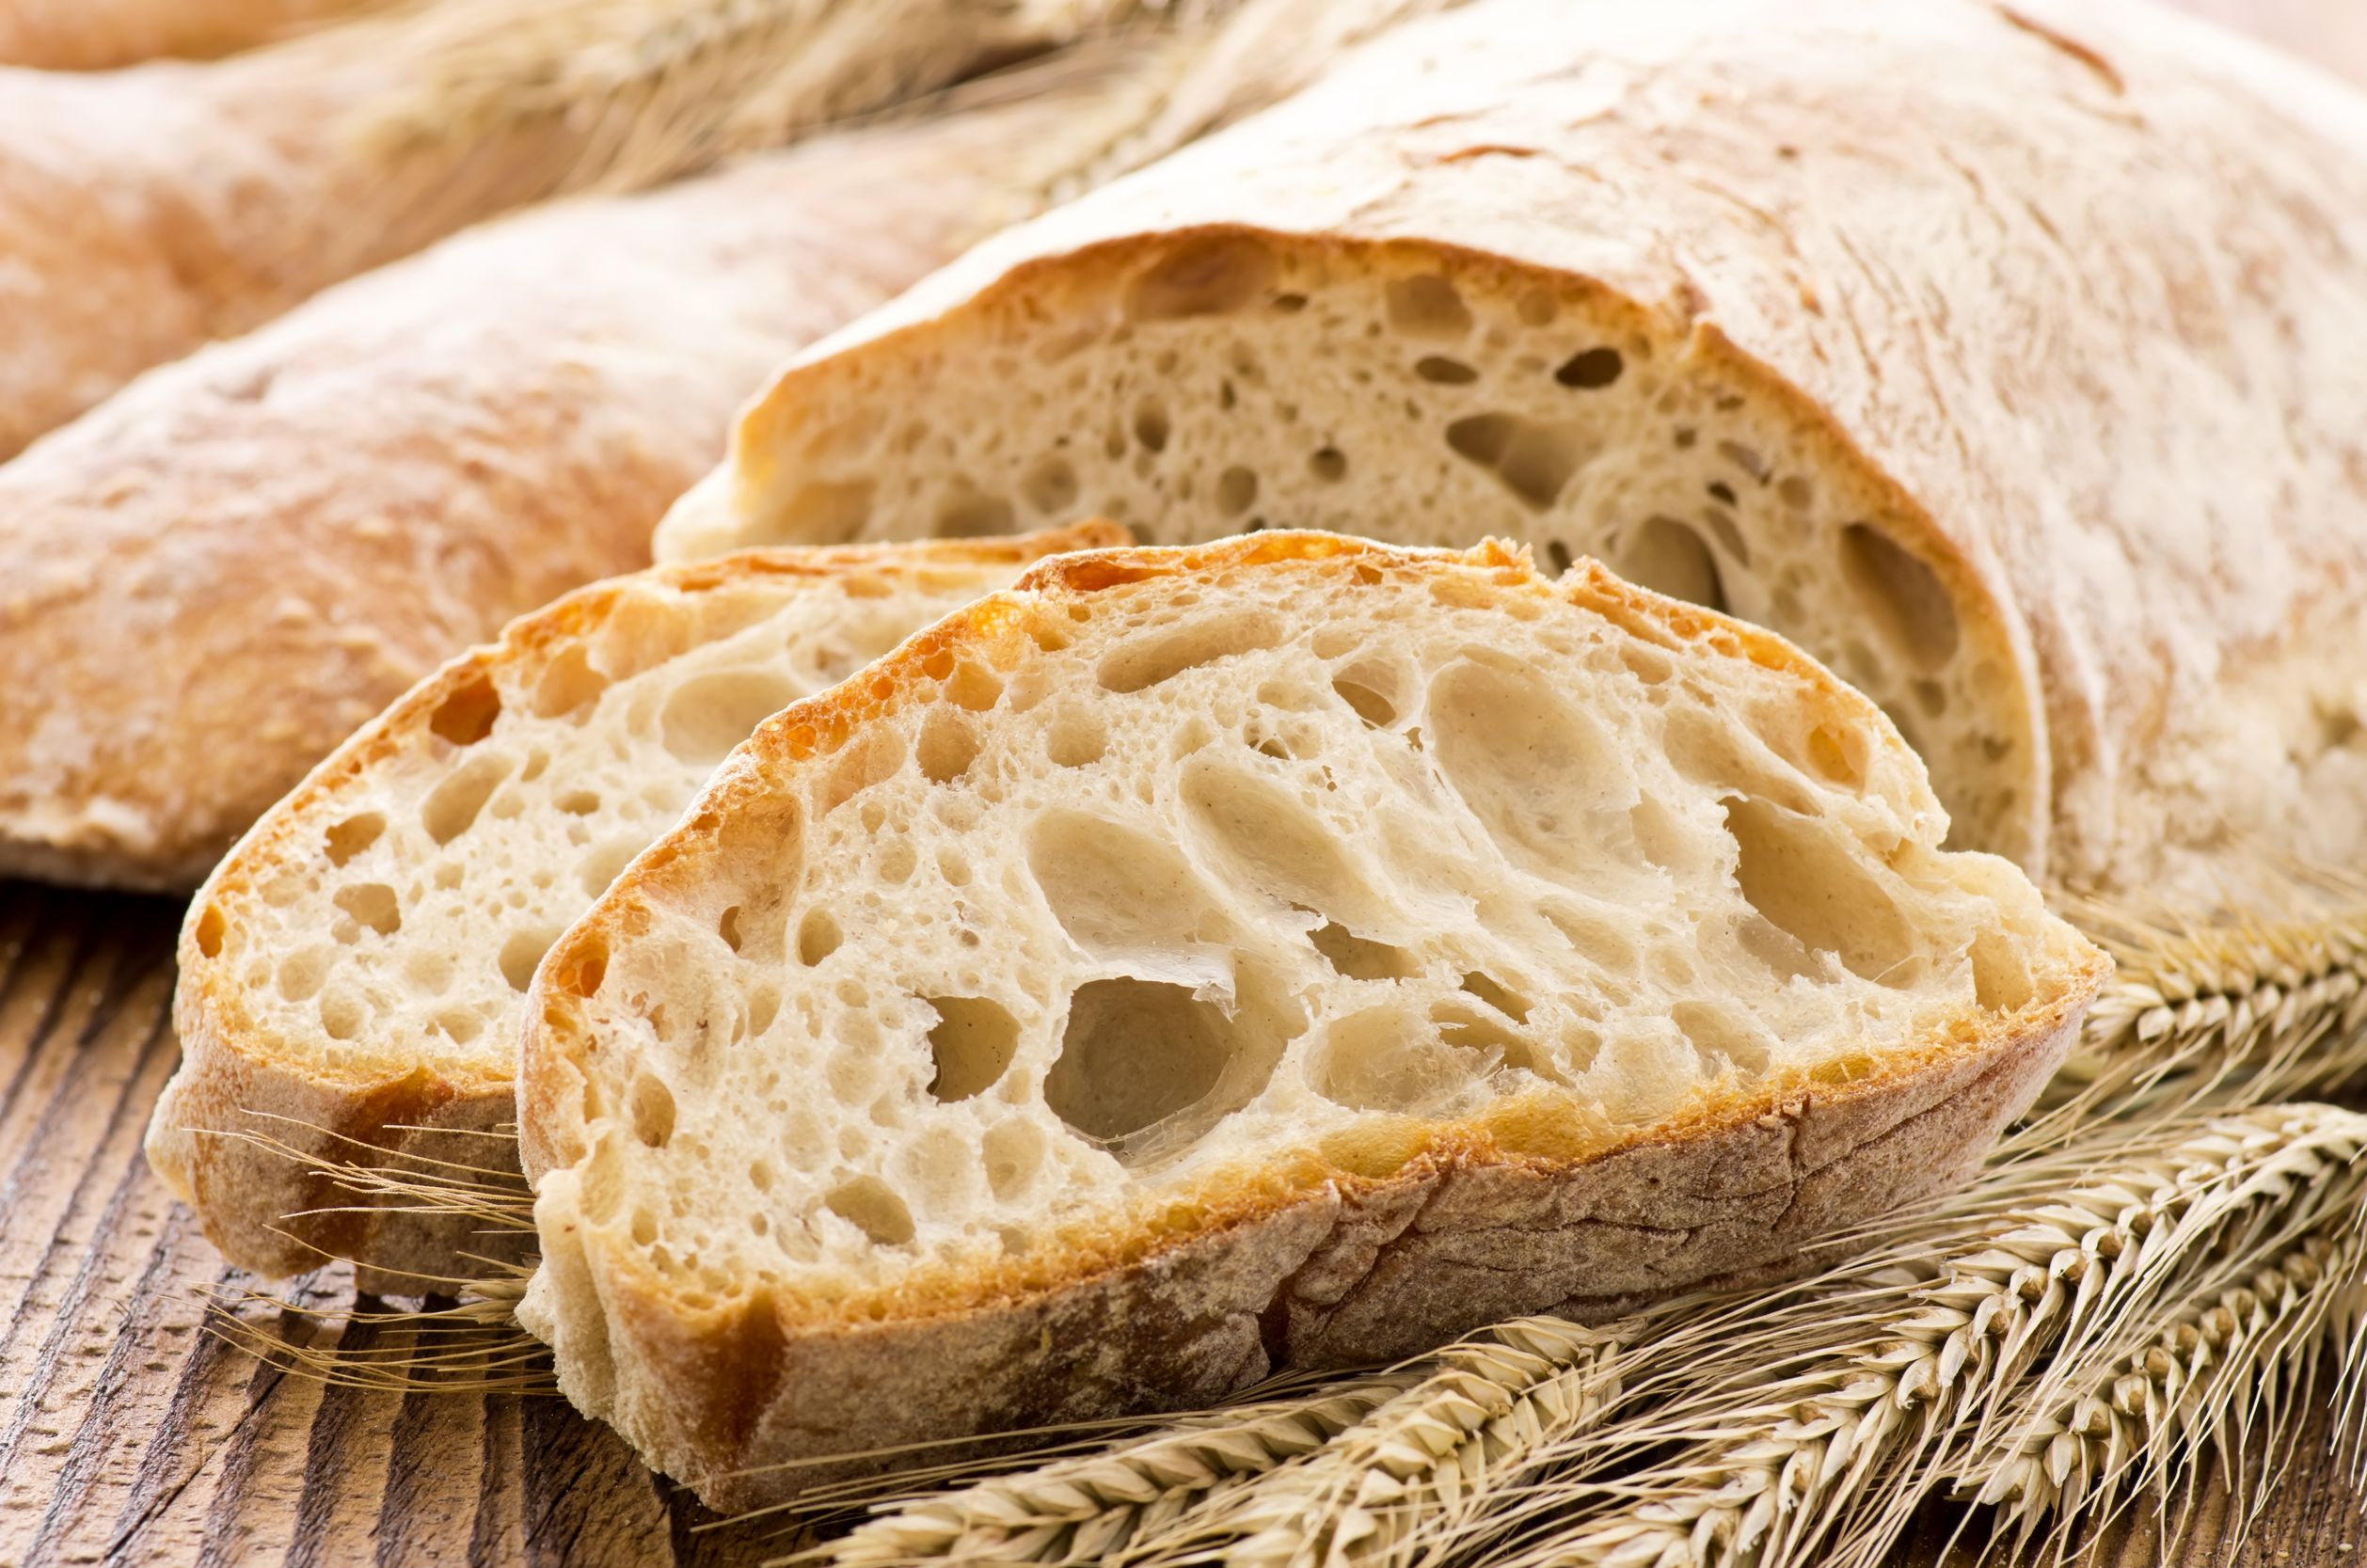
\includegraphics[width=\textwidth]{figures/bread.jpg}
	\end{column}
	\begin{column}{0.5\textwidth}
	\begin{itemize}
	\item Jesus used God as His basis for refuting Satan
	\item There is no objective morality without a God-provided standard
	\end{itemize}
	\end{column}
	\end{columns}
	
	\note{10:00}
	\note[item]{When God is `our' God, He sets the rules.}
	\note[item]{Jesus did not just quote any old verses from the Old Testament.}
	\note[item]{Every rebuttal was predicated on a respect for the greatness and authority of God.}
	\note[item]{Atheists, and indeed people in general, don't want an objective morality, until they become dissatisfied with their life}
	\note[item]{But, when we humble ourselves before God, we find refuge in the objective morality He provides.}
\end{frame}

\begin{frame}
	\frametitle{Love toward God is the foundation of eternal life}
	\framesubtitle{Luke 10:25-27}
	\begin{columns}
	\begin{column}{0.5\textwidth}
		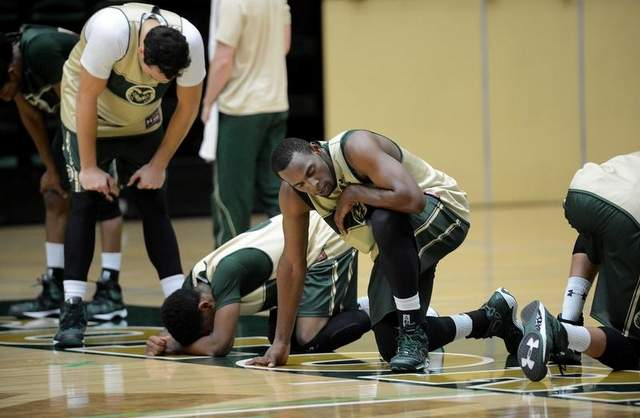
\includegraphics[width=\columnwidth]{figures/basketballRunning.jpg}
	\end{column}
	\begin{column}{0.5\textwidth}
		\begin{itemize}
			\item The main thing is to keep the main thing the main thing. -- {\footnotesize \emph{Steven Covey}}
			\item Sometimes we don't remember what giving all of ourselves looks like.
		\end{itemize}
	\end{column}
	\end{columns}
	\note{10:05}
	\note[item]{Loving God with all of ourselves is a `must have' for salvation.}
	\note[item]{We are not perfect.}
	\note[item]{In spite of that, though, we have to keep pushing.}
	\note[item]{Remember that we haven't given everything, yet.  We can always push to love God more.}
\end{frame}

\section{Review}

\begin{frame}
\frametitle{I will be their God}
\framesubtitle{God wants to be \emph{your} God}
\begin{columns}[c]
\begin{column}{0.3\textwidth}
	
\includegraphics[width=\columnwidth]{figures/uncleSam.jpg}
\end{column}
\begin{column}{0.7\textwidth}
	\begin{itemize}
		\item God is great and mighty
		\item God loves and blesses us.
		\item God shows Himself to man
		\item God's portrait is perfected in Jesus
		\item We meet Jesus in the Bible.  
		\item Respect for God can guide our lives
		\item Loving God is where salvation starts
	\end{itemize}
\end{column}
\end{columns}
\note{10:10}
\note[item]{Are you proud of being on God's team?}
\end{frame}

\chapter{They Shall be My People}

\begin{goals}
\goal God wants people who choose Him voluntarily.
\goal Understand the different ways God uses to call us to Him.
\goal Appreciate how unique and special a Christians' relationship with God is.
\end{goals}

\intro

\lipsum[4]

\bible

\begin{quote}
\lipsum[4] \bv{Jeremiah}{(31:31-33)}
\end{quote}

\begin{quote}
\lipsum[4] \bv{Jeremiah}{(31:31-33)}
\end{quote}

\begin{quote}
\lipsum[4] \bv{Jeremiah}{(31:31-33)}
\end{quote}

\begin{quote}
\lipsum[4] \bv{Jeremiah}{(31:31-33)}
\end{quote}

\discussion

\lipsum[5-7]

\questions

Question 1: Knowledge
\vfill

Question 2: Comprehension
\vfill

Question 3: Application
\vfill

Question 4: Analysis
\vfill

Question 5: Synthesis
\vfill

Question 6: Evaluation
\vfill

\chapter{The Covenant I Made With Their Fathers}

\begin{goals}
\goal Examine the role that covenants play in God's relationship with man
\goal Establish the importance of faith in both the Old and New Covenants
\goal Reflect on any ways that Christians could `return' to the weaknesses of Old Covenant
\end{goals}

\begin{bible}

\bvh{Genesis}{(6:17-18)}

17 ``Understand that I am bringing a flood -- floodwaters on the earth to destroy every creature under heaven with the breath of life in it. Everything on earth will die.  18 But I will establish My covenant with you, and you will enter the ark with your sons, your wife, and your sons' wives. 

\bvh{Galatians}{(3:1-29)}
3 You foolish Galatians! Who has hypnotized you, before whose eyes Jesus Christ was vividly portrayed as crucified?  2 I only want to learn this from you: Did you receive the Spirit by the works of the law or by hearing with faith?  3 Are you so foolish? After beginning with the Spirit, are you now going to be made complete by the flesh?  4 Did you suffer so much for nothing--if in fact it was for nothing?  5 So then, does God supply you with the Spirit and work miracles among you by the works of the law or by hearing with faith?

6 Just as Abraham believed God, and it was credited to him for righteousness,  7 then understand that those who have faith are Abraham's sons.  8 Now the Scripture saw in advance that God would justify the Gentiles by faith and told the good news ahead of time to Abraham, saying, All the nations will be blessed through you.  9 So those who have faith are blessed with Abraham, who had faith.

10 For all who rely on the works of the law are under a curse, because it is written: Everyone who does not continue doing everything written in the book of the law is cursed.  11 Now it is clear that no one is justified before God by the law, because the righteous will live by faith.  12 But the law is not based on faith; instead, the one who does these things will live by them.  13 Christ has redeemed us from the curse of the law by becoming a curse for us, because it is written: Everyone who is hung on a tree is cursed.  14 The purpose was that the blessing of Abraham would come to the Gentiles by Christ Jesus, so that we could receive the promised Spirit through faith.

15 Brothers, I'm using a human illustration. No one sets aside or makes additions to even a human covenant that has been ratified.  16 Now the promises were spoken to Abraham and to his seed. He does not say ``and to seeds,'' as though referring to many, but referring to one, and to your seed, who is Christ.  17 And I say this: The law, which came 430 years later, does not revoke a covenant that was previously ratified by God and cancel the promise.  18 For if the inheritance is from the law, it is no longer from the promise; but God granted it to Abraham through the promise.

19 Why then was the law given? It was added because of transgressions until the Seed to whom the promise was made would come. The law was put into effect through angels by means of a mediator.  20 Now a mediator is not for just one person, but God is one.  21 Is the law therefore contrary to God's promises? Absolutely not! For if a law had been given that was able to give life, then righteousness would certainly be by the law.  22 But the Scripture has imprisoned everything under sin's power, so that the promise by faith in Jesus Christ might be given to those who believe.  23 Before this faith came, we were confined under the law, imprisoned until the coming faith was revealed.  24 The law, then, was our guardian until Christ, so that we could be justified by faith.  25 But since that faith has come, we are no longer under a guardian,  26 for you are all sons of God through faith in Christ Jesus.

27 For as many of you as have been baptized into Christ have put on Christ like a garment.  28 There is no Jew or Greek, slave or free, male or female; for you are all one in Christ Jesus.  29 And if you belong to Christ, then you are Abraham's seed, heirs according to the promise. 

\end{bible}

\begin{discussion}

\dsubsec{Introduction}{900-905}{5}

\dsubsec{Examine the role that covenants play in God's relationship with man}{905-915}{10}

Genesis 6:17-18  God made a covenant with Noah

(Genesis 17:1-8) God made a Covenant with Abraham

Leviticus 26:1-45 God made a covenant with Israel

% This is actually used in lesson 08
Luke 22:14-23 Jesus' blood provides our New Covenant.  Same verse that Paul quotes in I Corinthians that we read for the Lord's Supper.

% probably need the Hebrews passage that says covenants are established with blood.

\dsubsec{Establish the importance of faith in both the Old and New Covenants}{915-925}{10}

Galatians 3:1-29 Even the Old Covenant was faith-based

Hebrews 11 The Hall of faith.

\dsubsec{Reflect on any ways that Christians could `return' to the Old Covenant.}{925-940}{15}

Back to Galatians.  Examine what it was that they were doing to 

\dsubsec{Review}{940-945}{5}
\end{discussion}

\begin{questions}
\q What is a covenant?
\q List all the covenants God has made with man through time.
\q Covenants usually have responsibilities for both parties involved.  For each covenant you listed in question 2, list God's responsibilities and man responsibilities.
\q Starting from Galatians 3:10-12 answer the following:  What role did faith play under the Old Covenant?
\end{questions}

\chapter{I Was Their Husband}

\begin{goals}
\goal Examine what it means for God to be a husband to His people.
\goal Elaborate on how God's love motivates us
\goal Consider practical ways to recognize and respond to God's love
\end{goals}

\begin{bible}
\bv{Genesis}{(2:20-24)}

20 The man gave names to all livestock and to the birds of the heavens and to every beast of the field. But for Adam there was not found a helper fit for him. 21 So the Lord God caused a deep sleep to fall upon the man, and while he slept took one of his ribs and closed up its place with flesh. 22 And the rib that the Lord God had taken from the man he made into a woman and brought her to the man. 23 Then the man said,
\begin{quote}
``This at last is bone of my bones and flesh of my flesh;\\
she shall be called Woman, because she was taken out of Man.”
\end{quote}
24 Therefore a man shall leave his father and his mother and hold fast to his wife, and they shall become one flesh

\bv{Hebrews}{(12:1-29)}
1 Therefore, since we are surrounded by so great a cloud of witnesses, let us also lay aside every weight, and sin which clings so closely, and let us run with endurance the race that is set before us, 2 looking to Jesus, the founder and perfecter of our faith, who for the joy that was set before him endured the cross, despising the shame, and is seated at the right hand of the throne of God.

3 Consider him who endured from sinners such hostility against himself, so that you may not grow weary or fainthearted. 4 In your struggle against sin you have not yet resisted to the point of shedding your blood. 5 And have you forgotten the exhortation that addresses you as sons?  ``My son, do not regard lightly the discipline of the Lord, nor be weary when reproved by him. 6 For the Lord disciplines the one he loves, and chastises every son whom he receives.''

7 It is for discipline that you have to endure. God is treating you as sons. For what son is there whom his father does not discipline? 8 If you are left without discipline, in which all have participated, then you are illegitimate children and not sons. 9 Besides this, we have had earthly fathers who disciplined us and we respected them. Shall we not much more be subject to the Father of spirits and live? 10 For they disciplined us for a short time as it seemed best to them, but he disciplines us for our good, that we may share his holiness. 11 For the moment all discipline seems painful rather than pleasant, but later it yields the peaceful fruit of righteousness to those who have been trained by it.

12 Therefore lift your drooping hands and strengthen your weak knees, 13 and make straight paths for your feet, so that what is lame may not be put out of joint but rather be healed. 14 Strive for peace with everyone, and for the holiness without which no one will see the Lord. 15 See to it that no one fails to obtain the grace of God; that no ``root of bitterness'' springs up and causes trouble, and by it many become defiled; 16 that no one is sexually immoral or unholy like Esau, who sold his birthright for a single meal. 17 For you know that afterward, when he desired to inherit the blessing, he was rejected, for he found no chance to repent, though he sought it with tears.

18 For you have not come to what may be touched, a blazing fire and darkness and gloom and a tempest 19 and the sound of a trumpet and a voice whose words made the hearers beg that no further messages be spoken to them. 20 For they could not endure the order that was given, ``If even a beast touches the mountain, it shall be stoned.'' 21 Indeed, so terrifying was the sight that Moses said, ``I tremble with fear.'' 22 But you have come to Mount Zion and to the city of the living God, the heavenly Jerusalem, and to innumerable angels in festal gathering, 23 and to the assembly of the firstborn who are enrolled in heaven, and to God, the judge of all, and to the spirits of the righteous made perfect, 24 and to Jesus, the mediator of a new covenant, and to the sprinkled blood that speaks a better word than the blood of Abel.

25 See that you do not refuse him who is speaking. For if they did not escape when they refused him who warned them on earth, much less will we escape if we reject him who warns from heaven. 26 At that time his voice shook the earth, but now he has promised, ``Yet once more I will shake not only the earth but also the heavens.'' 27 This phrase, ``Yet once more,'' indicates the removal of things that are shaken—that is, things that have been made—in order that the things that cannot be shaken may remain. 28 Therefore let us be grateful for receiving a kingdom that cannot be shaken, and thus let us offer to God acceptable worship, with reverence and awe, 29 for our God is a consuming fire.

\bv{IJohn}{(4:7-12)}
7 Beloved, let us love one another, for love is from God, and whoever loves has been born of God and knows God. 8 Anyone who does not love does not know God, because God is love. 9 In this the love of God was made manifest among us, that God sent his only Son into the world, so that we might live through him. 10 In this is love, not that we have loved God but that he loved us and sent his Son to be the propitiation for our sins. 11 Beloved, if God so loved us, we also ought to love one another. 12 No one has ever seen God; if we love one another, God abides in us and his love is perfected in us 
\end{bible}

\begin{discussion}

\dsubsec{Introduction}{900-905}{5}

\dsubsec{Examine what it means for God to be a husband to His people.}{905-915}{10}

Genesis 2:20-24 If you think that God does not intend to have a close relationship with you, this should dispel all doubt.

The most common metaphor for Israel was that of an unfaithful wife.

\dsubsec{Elaborate on how God's love motivates us}{915-925}{10}

Hebrews 12:1-29

\dsubsec{Consider practical ways to recognize and respond to God's love}{925-940}{15}

I John 4:7-12

\dsubsec{Review}{940-945}{5}
\end{discussion}

\chapter{My Covenant They Broke}

\begin{goals}
\goal Summarize how Israel rejected God's love under the Old Covenant
\goal Examine the consequences of rejecting God's love for Israel and for us
\goal Develop a plan to prevent falling away from God
\end{goals}

\begin{bible}

\bv{Hebrews}{(3:1-19)}

Therefore, holy brothers, you who share in a heavenly calling, consider Jesus, the apostle and high priest of our confession, 2 who was faithful to him who appointed him, just as Moses also was faithful in all God's house. 3 For Jesus has been counted worthy of more glory than Moses—as much more glory as the builder of a house has more honor than the house itself. 4 (For every house is built by someone, but the builder of all things is God.) 5 Now Moses was faithful in all God's house as a servant, to testify to the things that were to be spoken later, 6 but Christ is faithful over God's house as a son. And we are his house if indeed we hold fast our confidence and our boasting in our hope. 7 Therefore, as the Holy Spirit says, ``Today, if you hear his voice,8 do not harden your hearts as in the rebellion, on the day of testing in the wilderness, 9 where your fathers put me to the test and saw my works for forty years. 10 Therefore I was provoked with that generation, and said, `They always go astray in their heart; they have not known my ways.' 11 As I swore in my wrath, `They shall not enter my rest.' ''

12 Take care, brothers, lest there be in any of you an evil, unbelieving heart, leading you to fall away from the living God. 13 But exhort one another every day, as long as it is called ``today,'' that none of you may be hardened by the deceitfulness of sin. 14 For we have come to share in Christ, if indeed we hold our original confidence firm to the end. 15 As it is said, ``Today, if you hear his voice, do not harden your hearts as in the rebellion.'' 16 For who were those who heard and yet rebelled? Was it not all those who left Egypt led by Moses? 17 And with whom was he provoked for forty years? Was it not with those who sinned, whose bodies fell in the wilderness? 18 And to whom did he swear that they would not enter his rest, but to those who were disobedient? 19 So we see that they were unable to enter because of unbelief. 

\bv{Leviticus}{(26:1-45)}

``You shall not make idols for yourselves or erect an image or pillar, and you shall not set up a figured stone in your land to bow down to it, for I am the Lord your God. 2 You shall keep my Sabbaths and reverence my sanctuary: I am the Lord.

3 ``If you walk in my statutes and observe my commandments and do them, 4 then I will give you your rains in their season, and the land shall yield its increase, and the trees of the field shall yield their fruit. 5 Your threshing shall last to the time of the grape harvest, and the grape harvest shall last to the time for sowing. And you shall eat your bread to the full and dwell in your land securely. 6 I will give peace in the land, and you shall lie down, and none shall make you afraid. And I will remove harmful beasts from the land, and the sword shall not go through your land. 7 You shall chase your enemies, and they shall fall before you by the sword. 8 Five of you shall chase a hundred, and a hundred of you shall chase ten thousand, and your enemies shall fall before you by the sword. 9 I will turn to you and make you fruitful and multiply you and will confirm my covenant with you. 10 You shall eat old store long kept, and you shall clear out the old to make way for the new. 11 I will make my dwelling among you, and my soul shall not abhor you. 12 And I will walk among you and will be your God, and you shall be my people. 13 I am the Lord your God, who brought you out of the land of Egypt, that you should not be their slaves. And I have broken the bars of your yoke and made you walk erect.

14 ``But if you will not listen to me and will not do all these commandments, 15 if you spurn my statutes, and if your soul abhors my rules, so that you will not do all my commandments, but break my covenant, 16 then I will do this to you: I will visit you with panic, with wasting disease and fever that consume the eyes and make the heart ache. And you shall sow your seed in vain, for your enemies shall eat it. 17 I will set my face against you, and you shall be struck down before your enemies. Those who hate you shall rule over you, and you shall flee when none pursues you. 18 And if in spite of this you will not listen to me, then I will discipline you again sevenfold for your sins, 19 and I will break the pride of your power, and I will make your heavens like iron and your earth like bronze. 20 And your strength shall be spent in vain, for your land shall not yield its increase, and the trees of the land shall not yield their fruit.

21 ``Then if you walk contrary to me and will not listen to me, I will continue striking you, sevenfold for your sins. 22 And I will let loose the wild beasts against you, which shall bereave you of your children and destroy your livestock and make you few in number, so that your roads shall be deserted.

23 ``And if by this discipline you are not turned to me but walk contrary to me, 24 then I also will walk contrary to you, and I myself will strike you sevenfold for your sins. 25 And I will bring a sword upon you, that shall execute vengeance for the covenant. And if you gather within your cities, I will send pestilence among you, and you shall be delivered into the hand of the enemy. 26 When I break your supply of bread, ten women shall bake your bread in a single oven and shall dole out your bread again by weight, and you shall eat and not be satisfied.

27 ``But if in spite of this you will not listen to me, but walk contrary to me, 28 then I will walk contrary to you in fury, and I myself will discipline you sevenfold for your sins. 29 You shall eat the flesh of your sons, and you shall eat the flesh of your daughters. 30 And I will destroy your high places and cut down your incense altars and cast your dead bodies upon the dead bodies of your idols, and my soul will abhor you. 31 And I will lay your cities waste and will make your sanctuaries desolate, and I will not smell your pleasing aromas. 32 And I myself will devastate the land, so that your enemies who settle in it shall be appalled at it. 33 And I will scatter you among the nations, and I will unsheathe the sword after you, and your land shall be a desolation, and your cities shall be a waste.

34 ``Then the land shall enjoy its Sabbaths as long as it lies desolate, while you are in your enemies' land; then the land shall rest, and enjoy its Sabbaths. 35 As long as it lies desolate it shall have rest, the rest that it did not have on your Sabbaths when you were dwelling in it. 36 And as for those of you who are left, I will send faintness into their hearts in the lands of their enemies. The sound of a driven leaf shall put them to flight, and they shall flee as one flees from the sword, and they shall fall when none pursues. 37 They shall stumble over one another, as if to escape a sword, though none pursues. And you shall have no power to stand before your enemies. 38 And you shall perish among the nations, and the land of your enemies shall eat you up. 39 And those of you who are left shall rot away in your enemies' lands because of their iniquity, and also because of the iniquities of their fathers they shall rot away like them.

40 ``But if they confess their iniquity and the iniquity of their fathers in their treachery that they committed against me, and also in walking contrary to me, 41 so that I walked contrary to them and brought them into the land of their enemies—if then their uncircumcised heart is humbled and they make amends for their iniquity, 42 then I will remember my covenant with Jacob, and I will remember my covenant with Isaac and my covenant with Abraham, and I will remember the land. 43 But the land shall be abandoned by them and enjoy its Sabbaths while it lies desolate without them, and they shall make amends for their iniquity, because they spurned my rules and their soul abhorred my statutes. 44 Yet for all that, when they are in the land of their enemies, I will not spurn them, neither will I abhor them so as to destroy them utterly and break my covenant with them, for I am the Lord their God. 45 But I will for their sake remember the covenant with their forefathers, whom I brought out of the land of Egypt in the sight of the nations, that I might be their God: I am the Lord.''

\bv{Romans}{(9:30-33)}

30 What shall we say, then? That Gentiles who did not pursue righteousness have attained it, that is, a righteousness that is by faith; 31 but that Israel who pursued a law that would lead to righteousness did not succeed in reaching that law. 32 Why? Because they did not pursue it by faith, but as if it were based on works. They have stumbled over the stumbling stone, 33 as it is written,

\end{bible}

\begin{discussion}

\dsubsec{Introduction}{900-905}{5}

\dsubsec{Summarize how Israel rejected God's love under the Old Covenant}{905-915}{10}

Hebrews 3:1-19

Romans 9:30-33  Israel, as a nation,  didn't attain salvation through the Old Covenant because they did not pursue it by faith.

\dsubsec{Examine the consequences of rejecting God's love for Israel and for us}{915-925}{10}

Leviticus 26

\dsubsec{Develop a plan to prevent falling away from God}{925-940}{15}

Go back to Hebrews 3 and Romans 9

\dsubsec{Review}{940-945}{5}
\end{discussion}

\chapter{Behold The Days Are Coming}
\begin{goals}
\goal Know some prophecies from the Old Testament about the New Covenant
\goal Analyze how New Covenant prophesies set the expectations and hopes for the faithful of the Old Covenant
\goal Evaluate Bible prophecies that are not yet fulfilled, and the expectations and hopes they set for us6
\end{goals}
\begin{bible}

\bve{Genesis}{(22:15-19)}

15 And the angel of the Lord called to Abraham a second time from heaven 16 and said, ``By myself I have sworn, declares the Lord, because you have done this and have not withheld your son, your only son, 17 I will surely bless you, and I will surely multiply your offspring as the stars of heaven and as the sand that is on the seashore. And your offspring shall possess the gate of his enemies, 18 and in your offspring shall all the nations of the earth be blessed, because you have obeyed my voice.'' 19 So Abraham returned to his young men, and they arose and went together to Beersheba. And Abraham lived at Beersheba.

\bvh{Luke}{(2:22-40)}
22 And when the days of their purification according to the law of Moses were finished, they brought Him up to Jerusalem to present Him to the Lord 23 (just as it is written in the law of the Lord: Every firstborn male will be dedicated to the Lord) 24 and to offer a sacrifice (according to what is stated in the law of the Lord: a pair of turtledoves or two young pigeons).

25 There was a man in Jerusalem whose name was Simeon. This man was righteous and devout, looking forward to Israel's consolation, and the Holy Spirit was on him. 26 It had been revealed to him by the Holy Spirit that he would not see death before he saw the Lord's Messiah. 27 Guided by the Spirit, he entered the temple complex. When the parents brought in the child Jesus to perform for Him what was customary under the law, 28 Simeon took Him up in his arms, praised God, and said:
\begin{quote}
29 Now, Master, You can dismiss Your slave in peace, as You promised.
30 For my eyes have seen Your salvation.
31 You have prepared it in the presence of all peoples --
32 a light for revelation to the Gentiles and glory to Your people Israel.
\end{quote}
33 His father and mother were amazed at what was being said about Him. 34 Then Simeon blessed them and told His mother Mary: ``Indeed, this child is destined to cause the fall and rise of many in Israel and to be a sign that will be opposed— 35 and a sword will pierce your own soul—that the thoughts of many hearts may be revealed.''

36 There was also a prophetess, Anna, a daughter of Phanuel, of the tribe of Asher. She was well along in years, having lived with her husband seven years after her marriage, 37 and was a widow for 84 years. She did not leave the temple complex, serving God night and day with fasting and prayers. 38 At that very moment, she came up and began to thank God and to speak about Him to all who were looking forward to the redemption of Jerusalem.

39 When they had completed everything according to the law of the Lord, they returned to Galilee, to their own town of Nazareth. 40 The boy grew up and became strong, filled with wisdom, and God's grace was on Him.

\bvh{Romans}{(8:18-23)}

18 For I consider that the sufferings of this present time are not worth comparing with the glory that is going to be revealed to us. 19 For the creation eagerly waits with anticipation for God's sons to be revealed. 20 For the creation was subjected to futility--not willingly, but because of Him who subjected it--in the hope 21 that the creation itself will also be set free from the bondage of corruption into the glorious freedom of God's children. 22 For we know that the whole creation has been groaning together with labor pains until now. 23 And not only that, but we ourselves who have the Spirit as the firstfruits--we also groan within ourselves, eagerly waiting for adoption, the redemption of our bodies.

\end{bible}

\begin{discussion}

\dsubsec{Introduction}{900-905}{5}

\dsubsec{Know some prophecies from the Old Testament about the New Covenant}{905-915}{10}

\bvs{Genesis}{(22:15-19)} Land, nation, seed promises to Abraham 

Most of the prophecies are about Jesus.  No wonder they thought about a physical kingdom.  I'm going to have to think more on this.

\dsubsec{Analyze how New Covenant prophesies set the expectations and hopes for the faithful of the Old Covenant}{915-925}{10}

\bvs{Luke}{(2:22-40)} People who were expecting the coming of Christ

\dsubsec{Evaluate Bible prophecies that are not yet fulfilled, and the expectations and hopes they set for us}{925-940}{15}


\bvs{Romans}{(8:18-23)} Christians are still waiting for their coming glory.

\dsubsec{Review}{940-945}{5}
\end{discussion}

\begin{questions}
\q What is the relationship between Abraham's `seed' promise in Genesis 22:15-19 and the New Covenant prophecy in Jeremiah 31:31-34?
\q Compare the reaction of Anna and Simeon to Christ's coming to the reaction of the Pharisees later in Jesus' ministry.
\q Explain what Romans 8:19 means which it says that 'all creation' is waiting on God's sons to be revealed.
\q What are you looking forward to about Christ's second coming?
\end{questions}

\lecture{8. I Will Make a New Covenant}{08}

%------------------------------------------------------------------------------
\section{Introduction}
% this to put in this one:
% There is NO separation between church and personal life.
%--------------------------------------
\begin{frame}{IntroSlide}
\begin{center}
	
\includegraphics[draft, width=0.8\textwidth]{figures/dummy.png}
\end{center}

\note{09:30}
\end{frame}

%--------------------------------------
\begin{frame}{God wants a relationship with people}
\framesubtitle{Jeremiah 31:31-34}
	\keyversehiglight{I will make a new covenant}
	
\note{09:33}
\end{frame}

%--------------------------------------
\begin{goals}
\goal Examine what a husband is and how God is a husband to His people
\goal Elaborate on how God's love motivates us
\goal Consider practical ways to recognize and respond to God's love

\note{09:36}
\end{goals}

%------------------------------------------------------------------------------
\section{Section 1}

%--------------------------------------
\begin{frame}{Frame 1}
\framesubtitle{Passage 1}

\begin{columns}[c]
\begin{column}{0.6\textwidth}
	
\includegraphics[draft, width=\columnwidth]{figures/dummy.png}
\end{column}
\begin{column}{0.4\textwidth}
	Point 1\ldots
	\begin{itemize}
		\item Subpoint 1
	\end{itemize}
\end{column}
\end{columns}

\note{09:38}
\end{frame}

%------------------------------------------------------------------------------
\section{Section 2}

%------------------------------------------------------------------------------
\section{Section 3}

%------------------------------------------------------------------------------
\section{Review}

\begin{frame}{My covenant they broke}
	\begin{itemize}
		\item Goals
	\end{itemize}
	
\note{10:12}
\end{frame}



\chapter{Written On Their Hearts}

\begin{goals}
\goal Know what your `heart' is and how the New Covenant is `written' upon it
\goal Determine some internal and external ways to evaluate our hearts
\goal Commit to continual heart transformation as a way to draw closer to God
\end{goals}

\begin{bible}
\bve{ISamuel}{(16:7)}
7 But the Lord said to Samuel, ``Do not look on his appearance or on the height of his stature, because I have rejected him. For the Lord sees not as man sees: man looks on the outward appearance, but the Lord looks on the heart.''

\bvh{IICorinthians}{(4:16-18)}
16 Therefore we do not give up. Even though our outer person is being destroyed, our inner person is being renewed day by day. 17 For our momentary light affliction is producing for us an absolutely incomparable eternal weight of glory. 18 So we do not focus on what is seen, but on what is unseen. For what is seen is temporary, but what is unseen is eternal.

\bve{Ezra}{(7:10)}
For Ezra had set his heart to study the Law of the Lord, and to do it and to teach his statutes and rules in Israel.

\bve{Hebrews}{(4:1-13)}
Therefore, while the promise of entering his rest still stands, let us fear lest any of you should seem to have failed to reach it. 2 For good news came to us just as to them, but the message they heard did not benefit them, because they were not united by faith with those who listened. 3 For we who have believed enter that rest, as he has said,
\begin{quote}
``As I swore in my wrath,`They shall not enter my rest,'\thinspace''
\end{quote}
although his works were finished from the foundation of the world. 4 For he has somewhere spoken of the seventh day in this way: ``And God rested on the seventh day from all his works.'' 5 And again in this passage he said,
\begin{quote}
``They shall not enter my rest.''
\end{quote}
6 Since therefore it remains for some to enter it, and those who formerly received the good news failed to enter because of disobedience, 7 again he appoints a certain day, ``Today,'' saying through David so long afterward, in the words already quoted,
\begin{quote}
``Today, if you hear his voice, do not harden your hearts.''
\end{quote}
8 For if Joshua had given them rest, God would not have spoken of another day later on. 9 So then, there remains a Sabbath rest for the people of God, 10 for whoever has entered God's rest has also rested from his works as God did from his.

11 Let us therefore strive to enter that rest, so that no one may fall by the same sort of disobedience. 12 For the word of God is living and active, sharper than any two-edged sword, piercing to the division of soul and of spirit, of joints and of marrow, and discerning the thoughts and intentions of the heart. 13 And no creature is hidden from his sight, but all are naked and exposed to the eyes of him to whom we must give account.

\bve{IJohn}{(3:19-24)}
19 By this we shall know that we are of the truth and reassure our heart before him; 20 for whenever our heart condemns us, God is greater than our heart, and he knows everything. 21 Beloved, if our heart does not condemn us, we have confidence before God; 22 and whatever we ask we receive from him, because we keep his commandments and do what pleases him. 23 And this is his commandment, that we believe in the name of his Son Jesus Christ and love one another, just as he has commanded us. 24 Whoever keeps his commandments abides in God, and God in him. And by this we know that he abides in us, by the Spirit whom he has given us.

\bvh{Romans}{(12:1-2)}
1 Therefore, brothers, by the mercies of God, I urge you to present your bodies as a living sacrifice, holy and pleasing to God; this is your spiritual worship. 2 Do not be conformed to this age, but be transformed by the renewing of your mind, so that you may discern what is the good, pleasing, and perfect will of God.

\bve{Ephesians}{(3:14-18)}
14 For this reason I bow my knees before the Father, 15 from whom every family in heaven and on earth is named, 16 that according to the riches of his glory he may grant you to be strengthened with power through his Spirit in your inner being, 17 so that Christ may dwell in your hearts through faith—that you, being rooted and grounded in love, 18 may have strength to comprehend with all the saints what is the breadth and length and height and depth,

\bvh{Philippians}{(3:3-10)}
1 For we are the circumcision, the ones who serve by the Spirit of God, boast in Christ Jesus, and do not put confidence in the flesh-- 4 although I once also had confidence in the flesh. If anyone else thinks he has grounds for confidence in the flesh, I have more: 5 circumcised the eighth day; of the nation of Israel, of the tribe of Benjamin, a Hebrew born of Hebrews; regarding the law, a Pharisee; 6 regarding zeal, persecuting the church; regarding the righteousness that is in the law, blameless.

7 But everything that was a gain to me, I have considered to be a loss because of Christ. 8 More than that, I also consider everything to be a loss in view of the surpassing value of knowing Christ Jesus my Lord. Because of Him I have suffered the loss of all things and consider them filth, so that I may gain Christ 9 and be found in Him, not having a righteousness of my own from the law, but one that is through faith in Christ--the righteousness from God based on faith. 10 My goal is to know Him and the power of His resurrection and the fellowship of His sufferings, being conformed to His death,

\end{bible}

\begin{discussion}
\dsubsec{Introduction}{900-905}{5}

Written on their hearts as opposed to simply written on tablets of stone.

The heart is `soft' as opposed to `hard'.  Appreciate in what ways our heart can be measured.

\dsubsec{Know what your `heart' is and how the New Covenant is `written' upon it}{905-915}{10}

\bvs{ISamuel}{(16:7)} Man looks at the outward appearance.  God looks at the heart

\bvs{IICorinthians}{(4:16-18)} The inner part of us that can be renewed

\bvs{Ezra}{(7:10)} Ezra chose what His heart would be like.

\bvs{Deuteronomy}{(10:12-22)} Lesson 3.  God demands our hearts.

\dsubsec{Appreciate the internal and external ways to evaluate our hearts}{915-925}{10}

\bvs{Hebrews}{(4:1-13)} Don't have the Isaelites' heart, but have faith guided by God's Word.

And, it's supposed not only to govern our outward behavior, but also how we feel and think.

\bvs{IJohn}{(3:19-24)} A heart that has love and obedience gives us confidence.\\

\dsubsec{Commit to continual heart transformation as a way to draw closer to God}{925-940}{15}

\bvs{Ezra}{(7:10)} We can choose which way it will go

\bvs{Romans}{(12:1-2)} Christians commit to a total life transformation.

\bvs{Ephesians}{(3:14-18)} Our hearts is strengthened when we understand God's love

% This is a candidate for moving
\bvs{Philippians}{(3:3-10)} We are the circumcision, and focus our lives on knowing Christ.

\dsubsec{Review}{940-945}{5}
\end{discussion}

\begin{questions}
\q What is your heart as it's used in the Bible?
\q List some of the ways that Hebrews 4:1-13 teaches us to avoid having a heart like the Israelites.
\q Think of a theme, intimately tied to our hearts, that connect Ephesians 3:14-18, Deuteronomy 10:12-22, and I John 3:19-24.
\q Think of a few practical ways that you can change your own heart in order to grow in your relationship with God.
\end{questions}

\chapter{For They Shall All Know Me}

\begin{goals}
\goal Show that God's people are now joined by a common faith not a common ancestry 
\goal Elaborate on what it means to `know' God
\goal Come up with a plan to know God better
\end{goals}

\begin{bible}
\bve{Romans}{(4:1-25)}
What then shall we say was gained by Abraham, our forefather according to the flesh? 2 For if Abraham was justified by works, he has something to boast about, but not before God. 3 For what does the Scripture say? ``Abraham believed God, and it was counted to him as righteousness.'' 4 Now to the one who works, his wages are not counted as a gift but as his due. 5 And to the one who does not work but believes in him who justifies the ungodly, his faith is counted as righteousness, 6 just as David also speaks of the blessing of the one to whom God counts righteousness apart from works:
\begin{quote}
7 ``Blessed are those whose lawless deeds are forgiven, and whose sins are covered;
8 blessed is the man against whom the Lord will not count his sin.''
\end{quote}
9 Is this blessing then only for the circumcised, or also for the uncircumcised? For we say that faith was counted to Abraham as righteousness. 10 How then was it counted to him? Was it before or after he had been circumcised? It was not after, but before he was circumcised. 11 He received the sign of circumcision as a seal of the righteousness that he had by faith while he was still uncircumcised. The purpose was to make him the father of all who believe without being circumcised, so that righteousness would be counted to them as well, 12 and to make him the father of the circumcised who are not merely circumcised but who also walk in the footsteps of the faith that our father Abraham had before he was circumcised.

13 For the promise to Abraham and his offspring that he would be heir of the world did not come through the law but through the righteousness of faith. 14 For if it is the adherents of the law who are to be the heirs, faith is null and the promise is void. 15 For the law brings wrath, but where there is no law there is no transgression.

16 That is why it depends on faith, in order that the promise may rest on grace and be guaranteed to all his offspring--not only to the adherent of the law but also to the one who shares the faith of Abraham, who is the father of us all, 17 as it is written, ``I have made you the father of many nations''--in the presence of the God in whom he believed, who gives life to the dead and calls into existence the things that do not exist. 18 In hope he believed against hope, that he should become the father of many nations, as he had been told, ``So shall your offspring be.'' 19 He did not weaken in faith when he considered his own body, which was as good as dead (since he was about a hundred years old), or when he considered the barrenness of Sarah's womb. 20 No unbelief made him waver concerning the promise of God, but he grew strong in his faith as he gave glory to God, 21 fully convinced that God was able to do what he had promised. 22 That is why his faith was ``counted to him as righteousness.'' 23 But the words ``it was counted to him'' were not written for his sake alone, 24 but for ours also. It will be counted to us who believe in him who raised from the dead Jesus our Lord, 25 who was delivered up for our trespasses and raised for our justification.

\bvh{Philippians}{(3:3-10)}
1 For we are the circumcision, the ones who serve by the Spirit of God, boast in Christ Jesus, and do not put confidence in the flesh-- 4 although I once also had confidence in the flesh. If anyone else thinks he has grounds for confidence in the flesh, I have more: 5 circumcised the eighth day; of the nation of Israel, of the tribe of Benjamin, a Hebrew born of Hebrews; regarding the law, a Pharisee; 6 regarding zeal, persecuting the church; regarding the righteousness that is in the law, blameless.

7 But everything that was a gain to me, I have considered to be a loss because of Christ. 8 More than that, I also consider everything to be a loss in view of the surpassing value of knowing Christ Jesus my Lord. Because of Him I have suffered the loss of all things and consider them filth, so that I may gain Christ 9 and be found in Him, not having a righteousness of my own from the law, but one that is through faith in Christ--the righteousness from God based on faith. 10 My goal is to know Him and the power of His resurrection and the fellowship of His sufferings, being conformed to His death,

\bve{Ephesians}{(3:14-18)}
14 For this reason I bow my knees before the Father, 15 from whom every family in heaven and on earth is named, 16 that according to the riches of his glory he may grant you to be strengthened with power through his Spirit in your inner being, 17 so that Christ may dwell in your hearts through faith--that you, being rooted and grounded in love, 18 may have strength to comprehend with all the saints what is the breadth and length and height and depth,

\bvh{Matthew}{(7:7-12)}
7 ``Keep asking, and it will be given to you. Keep searching, and you will find. Keep knocking, and the door will be opened to you. 8 For everyone who asks receives, and the one who searches finds, and to the one who knocks, the door will be opened. 9 What man among you, if his son asks him for bread, will give him a stone? 10 Or if he asks for a fish, will give him a snake? 11 If you then, who are evil, know how to give good gifts to your children, how much more will your Father in heaven give good things to those who ask Him! 12 Therefore, whatever you want others to do for you, do also the same for them--this is the Law and the Prophets.

\end{bible}

\begin{discussion}
\dsubsec{Introduction}{900-905}{5}

\dsubsec{Show that God's people are now joined by a common faith not a common ancestry }{905-915}{10}

\bvs{Romans}{(4:1-25)} Those who have the faith of Abraham are his children.

\bvs{Phil}{(3:3-10)} Lesson 9. also says we are the true circumcision.

\dsubsec{Elaborate on what it means to `know' God}{915-925}{10}

These passages emphasize the importance of knowing God, but not necessarily what there is to know!.
\bvs{Ephesians}{(3:14-18)} Lesson 9

\dsubsec{Come up with a plan to know God better}{925-940}{15}

\bvs{Matthew}{(7:7-12)} Keep asking and it will be given you.

\dsubsec{Review}{940-945}{5}
\end{discussion}

\begin{questions}
\q Thinking about Romans 4, interpret the phrase ``For they shall \emph{all} know me'' from Jeremiah 31:34
\q Explain the weakness of God's special people being based on physical genealogy under the Old Covenant.
\q Given that Christians are now God's special people, what should we focus on according to Philippians 3:3-10 and Ephesians 3:14-18.
\q List four practical you could try to know God better.
\end{questions}

\chapter{From the Least to the Greatest}

\begin{goals}
% worldy churches do a lot for improving the lives of their fellow man, but we don't do that.
\goal Review the separation that existing under the Old Law between God and His people 
\goal Appreciate the breadth of people that make up the New Testament church
\goal Propose godly ways we can enhance the inclusiveness of the Lord's church
\end{goals}

\begin{bible}

\bve{Hebrews}{(9:1-14)}
1 Now even the first covenant had regulations for worship and an earthly place of holiness. 2 For a tent was prepared, the first section, in which were the lampstand and the table and the bread of the Presence. It is called the Holy Place. 3 Behind the second curtain was a second section called the Most Holy Place, 4 having the golden altar of incense and the ark of the covenant covered on all sides with gold, in which was a golden urn holding the manna, and Aaron's staff that budded, and the tablets of the covenant. 5 Above it were the cherubim of glory overshadowing the mercy seat. Of these things we cannot now speak in detail.

6 These preparations having thus been made, the priests go regularly into the first section, performing their ritual duties, 7 but into the second only the high priest goes, and he but once a year, and not without taking blood, which he offers for himself and for the unintentional sins of the people. 8 By this the Holy Spirit indicates that the way into the holy places is not yet opened as long as the first section is still standing 9 (which is symbolic for the present age). According to this arrangement, gifts and sacrifices are offered that cannot perfect the conscience of the worshiper, 10 but deal only with food and drink and various washings, regulations for the body imposed until the time of reformation.

11 But when Christ appeared as a high priest of the good things that have come, then through the greater and more perfect tent (not made with hands, that is, not of this creation) 12 he entered once for all into the holy places, not by means of the blood of goats and calves but by means of his own blood, thus securing an eternal redemption. 13 For if the blood of goats and bulls, and the sprinkling of defiled persons with the ashes of a heifer, sanctify for the purification of the flesh, 14 how much more will the blood of Christ, who through the eternal Spirit offered himself without blemish to God, purify our conscience from dead works to serve the living God.

\bve{Ephesians}{(3:1-6)}
1 For this reason I, Paul, a prisoner for Christ Jesus on behalf of you Gentiles— 2 assuming that you have heard of the stewardship of God's grace that was given to me for you, 3 how the mystery was made known to me by revelation, as I have written briefly. 4 When you read this, you can perceive my insight into the mystery of Christ, 5 which was not made known to the sons of men in other generations as it has now been revealed to his holy apostles and prophets by the Spirit. 6 This mystery is that the Gentiles are fellow heirs, members of the same body, and partakers of the promise in Christ Jesus through the gospel.

\bve{Matthew}{(20:1-16)}

1 ``For the kingdom of heaven is like a master of a house who went out early in the morning to hire laborers for his vineyard. 2 After agreeing with the laborers for a denarius a day, he sent them into his vineyard. 3 And going out about the third hour he saw others standing idle in the marketplace, 4 and to them he said, ‘You go into the vineyard too, and whatever is right I will give you.’ 5 So they went. Going out again about the sixth hour and the ninth hour, he did the same. 6 And about the eleventh hour he went out and found others standing. And he said to them, ‘Why do you stand here idle all day?’ 7 They said to him, ‘Because no one has hired us.’ He said to them, ‘You go into the vineyard too.’ 8 And when evening came, the owner of the vineyard said to his foreman, ‘Call the laborers and pay them their wages, beginning with the last, up to the first.’ 9 And when those hired about the eleventh hour came, each of them received a denarius. 10 Now when those hired first came, they thought they would receive more, but each of them also received a denarius. 11 And on receiving it they grumbled at the master of the house, 12 saying, ‘These last worked only one hour, and you have made them equal to us who have borne the burden of the day and the scorching heat.’ 13 But he replied to one of them, ‘Friend, I am doing you no wrong. Did you not agree with me for a denarius? 14 Take what belongs to you and go. I choose to give to this last worker as I give to you. 15 Am I not allowed to do what I choose with what belongs to me? Or do you begrudge my generosity?’ 16 So the last will be first, and the first last.''

\bvh{Ephesians}{(4:1-16)}
1 Therefore I, the prisoner for the Lord, urge you to walk worthy of the calling you have received, 2 with all humility and gentleness, with patience, accepting one another in love, 3 diligently keeping the unity of the Spirit with the peace that binds us. 4 There is one body and one Spirit--just as you were called to one hope at your calling-- 5 one Lord, one faith, one baptism, 6 one God and Father of all, who is above all and through all and in all.

7 Now grace was given to each one of us according to the measure of the Messiah's gift. 8 For it says:
\begin{quote}
When He ascended on high,
He took prisoners into captivity;
He gave gifts to people.
\end{quote}
9 But what does ``He ascended'' mean except that He descended to the lower parts of the earth? 10 The One who descended is also the One who ascended far above all the heavens, that He might fill all things. 11 And He personally gave some to be apostles, some prophets, some evangelists, some pastors and teachers, 12 for the training of the saints in the work of ministry, to build up the body of Christ, 13 until we all reach unity in the faith and in the knowledge of God's Son, growing into a mature man with a stature measured by Christ's fullness. 14 Then we will no longer be little children, tossed by the waves and blown around by every wind of teaching, by human cunning with cleverness in the techniques of deceit. 15 But speaking the truth in love, let us grow in every way into Him who is the head--Christ. 16 From Him the whole body, fitted and knit together by every supporting ligament, promotes the growth of the body for building up itself in love by the proper working of each individual part.

\bvg{James}{(2:1-7)}
My brothers, do not show favoritism as you hold on to the faith in our glorious Lord Jesus Christ. 2 For example, a man comes into your meeting wearing a gold ring and dressed in fine clothes, and a poor man dressed in dirty clothes also comes in. 3 If you look with favor on the man wearing the fine clothes and say, ``Sit here in a good place,'' and yet you say to the poor man, ``Stand over there,'' or, ``Sit here on the floor by my footstool,'' 4 haven't you discriminated among yourselves and become judges with evil thoughts?

5 Listen, my dear brothers: Didn't God choose the poor in this world to be rich in faith and heirs of the kingdom that He has promised to those who love Him? 6 Yet you dishonored that poor man. Don’t the rich oppress you and drag you into the courts? 7 Don't they blaspheme the noble name that was pronounced over you at your baptism?

\end{bible}

\begin{discussion}
\dsubsec{Introduction}{900-905}{5}

\dsubsec{Review the separation that existing under the Old Law between God and His people }{905-915}{10}

\bvs{Hebrews}{(9:1-14)} The tabernacle separated the Israelites from God.

\bvs{Ephesians}{(3:1-6)} The mystery of the Gospel is that Gentiles can enter heaven.

\dsubsec{Appreciate the breadth of people that make up the New Testament church}{915-925}{10}

\bvs{Matthew}{(20:1-16)} Early or late

Corinthians not many wise.

\dsubsec{Propose godly ways we can enhance the inclusiveness of the Lord's church}{925-940}{15}

\bvs{Ephesians}{(4:1-16)} Christians are each part of a body, and work toward unity.

\bvs{James}{(2:1-7)} The church is made up of both rich and poor

\dsubsec{Review}{940-945}{5}
\end{discussion}

\begin{questions}
\q What is the mystery of the Gospel?
\q List some of the different types of people that could conflict with each other, but who must get along in the church (for example, rich and poor).
\q Paul lists some of the specific teaching roles that Ephesian Christians held (apostles, prophets, evangelists, pastors and teachers), but there are other areas where Christians may have personal strengths that are helpful to the body of Christ.  List as many as you can think of.
\q What areas could we improve on to increase the inclusiveness of the Lord's church?
\end{questions}

\lecture{12. I Will Forgive Their Iniquity}{12}

%------------------------------------------------------------------------------
\section{Introduction}

%--------------------------------------
\begin{frame}{God wants to have mercy on all}

\begin{center}

\includegraphics[height=0.8\textheight]{figures/ladyJustice.jpg}
\end{center}

\note{09:00}
\note[item]{This depiction of lady justice illustrates a few things we'd like to avoid when it comes to our spiritual life.}
\note[item]{The balance: What you've done will be weighed exactly against the standard.}
\note[item]{The blindfold: You can't get out of it because you're special.}
\note[item]{The sword: If the balance finds you guilty, consequences will follow.}
\note[item]{But, God arranged His plan specifically so He could show mercy}
\note[item]{It's hard for us to understand, because we're used to how our justice system works.}
\note[item]{Governments seek out the wrong-doers for the expressed purpose of bringing them to justice.}
\note[item]{Our Lord sought out wrong-doers to help them avoid the justice they deserve.}
\end{frame}



%--------------------------------------
\begin{frame}{God wants a relationship with people}
\framesubtitle{Jeremiah 31:31-34}
	\keyversehiglight{For I will forgive their iniquity, and I will remember their sin no more.}
\note{09:33}
\end{frame}

%--------------------------------------
\begin{goals}
\goal Know what sin is, why it separates us from God, and what God has done about it in the New Covenant
\goal Examine why it is easy for us to strive for perfect lawkeeping rather than faithfulness
\goal Consider ways to keep the guilt of past sins from damaging your current relationship with God

\note{09:35}
\end{goals}

%------------------------------------------------------------------------------
\section{Sin is everyone's problem}

%--------------------------------------
\begin{frame}{Law shows us what's right and wrong}
\framesubtitle{Romans 3:5-28}

\begin{itemize}
	\item Law brings a knowledge right and wrong
	\item We become aware of our sin.
	\item ``Men and brethren, what should we do?''
\end{itemize}

\note{09:38}
\end{frame}

%--------------------------------------
\begin{frame}{God's plan shows mercy to everyone}
\framesubtitle{Romans 3:5-28}

\begin{itemize}
	\item God is the judge
	\item He's also the only one who could provide a solution to sin.
	\item Thus, he is both just and justifier
	\item Under his New plan\ldots
	\begin{itemize}
		\item there is no room for boasting
		\item we live under a law of faith
		\item the law of works is satisfied
	\end{itemize}
\end{itemize}

\note{09:42}
\end{frame}

%--------------------------------------
\begin{frame}{Jesus is God's solution to sin.}
\framesubtitle{Hebrews 9:15-28}

\begin{itemize}
\item Jesus blood was a necessary condition for the New Covenant.
\item Jesus' death took care of sin once for all.
\item When he comes back he won't have to deal with sin again, but rather will deal with salvation.
\end{itemize}

\note{09:46}
\end{frame}

%------------------------------------------------------------------------------
\section{The importance of faithfulness}

\begin{frame}
\frametitle{`The Law' is both a thing and an idea}
\begin{center}

\includegraphics[width=0.8\textwidth]{figures/law.jpg}\\
The thing: The written Law of Moses\\
The idea: Justification through a system of works
\end{center}

\note{09:50}
\note[item]{We sometimes try to shoehorn every instance of the word `law' into meaning simply the Law of Moses.}
\note[item]{Why do we do that? Because there are many so-called `Christians' who would say that you don't have to do good works to go to heaven.}
\note[item]{These people misunderstand the word `law' to mean that \emph{any} attempt to do good works is futile and has no bearing on whether or not you enter heaven.}
\note[item]{So, to combat that, we say, `Well, these passages are talking about the Law of Moses, not just doing good works in general'.}
\note[item]{But, if we treat the word `law' as meaning simply the Law of Moses, we are taking large chunks of the New Testament and saying, ``That doesn't apply to me.''}
\note[item]{Paul in particularly uses the term `law' to fill a bigger concept.  And, it \emph{does}, I believe, have application for us.}
\end{frame}

%--------------------------------------
\begin{frame}{Life is hard for those who want to do right}
\framesubtitle{Romans 7:1-25}
\begin{itemize}
	\item There's always a conflict between the flesh and the spirit
	\item If you're in Christ, you'd like to \emph{never} sin.
	\item But, that doesn't happen.
	\item So, what do we do?
\end{itemize}
\note{09:55}
\end{frame}

%------------------------------------------------------------------------------
\section{Letting go of sin}

%--------------------------------------
\begin{frame}{There is no condemnation}
\framesubtitle{Romans 8:1-11}
\begin{itemize}
\item No condemnation exists for those in Christ
\item You are set free from sin
\item The requirements of the law are fulfilled in those who walk not in the flesh, but in the Spirit.
\end{itemize}

\note{10:00}
\end{frame}

%--------------------------------------
\begin{frame}{Faithfulness not perfection}
\framesubtitle{Hebrews 11:1}

\begin{itemize}
\item Faith \emph{is} our assurance.
\item Faith \emph{is} our conviction.
\item You have to trust God that he's forgiven your sins.
\item How do I get that faith? (Rom. 10:17)
\end{itemize}

\note{10:05}
\end{frame}

%------------------------------------------------------------------------------
\section{Review}

\begin{frame}{I Will Forgive Their Sins}
Sin separates us from God.
\begin{itemize}
	\item Law shows us what's right and wrong
	\item God's plan forgives our sins\ldots
	\item And, keeps Him just.
	\item The plan required the blood of Jesus
\end{itemize}
Our lack of perfection is frustrating
\begin{itemize}
	\item People who love God want to do what's right
	\item But we can be frustrated because we're not perfect.
	\item Jesus is the solution to those problems, too.
\end{itemize}
Have faith in your forgiveness
\begin{itemize}
	\item \emph{No} condemnation exists for those in Christ.
	\item You have to trust God.
	\item Bolster your faith through the Word.
\end{itemize}
	
\note{10:10}
\end{frame}


\chapter{Review}

\begin{goals}
\goal See Class Objectives on page \pageref{sec:ClassObjectives}
\end{goals}
\begin{bible}
Review Jeremiah 31:31-34 on page \pageref{sec:KeyPassage}.
\end{bible}

\begin{discussion}
\dsubsec{Introduction}{900-905}{5}
Question about whether sin exists or not? Most people who don't believe in God, don't believe in sin either.
We are in the business of faithfulness, not perfect lawkeeping

\dsubsec{The big picture of the bible}{905-915}{10}
God wants a relationship with a holy people who voluntarily choose Him

\dsubsec{Relationship theme Old to New}{915-925}{10}

\dsubsec{Develop your own relationship}{925-940}{15}

\dsubsec{Review}{940-945}{5}

\end{discussion}

\begin{questions}
\q Pick three passages used in this class that have had the greatest impact on you and explain why they were meaningful to you.
\q Summarize the message of Jeremiah 31:31-34
\q Explain why developing an actual relationship with God is important.
\q How will you continue to grow your relationship with God?
\end{questions}

\appendix
\backmatter

\end{document}